\section{Phân tích hệ thống}
\subsection{Stakeholders}
\subsubsection{Đội phát triển phần mềm}

Nhóm phát triển phần mềm chịu trách nhiệm xây dựng, thử nghiệm và triển khai sản phẩm theo các yêu cầu được cung cấp.

\begin{itemize}
    \item \textbf{Nhu cầu:}
    \begin{itemize}
        \item Nhóm cần có phạm vi dự án và các yêu cầu được xác định rõ ràng để đảm bảo lập kế hoạch hiệu quả và đồng nhất với các mục tiêu được đặt ra.
        \item Nhóm cần được tạo điều kiện tiếp cận các công cụ và công nghệ cần thiết để thực hiện nhiệm vụ của mình một cách hiệu quả và sáng tạo.
    \end{itemize}
    \item \textbf{Ảnh hưởng:} Nhóm phát triển có ảnh hưởng lớn do nhóm tham gia trực tiếp vào quá trình thực hiện dự án. Công việc của nhóm tác động trực tiếp đến chất lượng và chức năng của sản phẩm cuối cùng, khiến cho sự đóng góp và sự hài lòng của nhóm phát triển quan trọng đối với sự thành công của dự án.
\end{itemize}

\subsubsection{Các doanh nghiệp khách hàng}

Đây là những doanh nghiệp sử dụng hệ thống để tạo và triển khai chatbot AI trên trang web của họ.

\begin{itemize}
    \item \textbf{Nhu cầu:}
    \begin{itemize}
        \item Khách hàng cần một giao diện trực quan và tích hợp liền mạch để tăng hiệu quả và giảm thiểu thời gian triển khai.
        \item Chatbot cần có khả năng tùy chỉnh giao diện để phù hợp với nhận diện thương hiệu của khách hàng.
        \item Chức năng của chatbot cần đáng tin cậy và hiệu suất cao để duy trì sự hài lòng của người dùng.
        \item Hệ thống cần đảm bảo bảo vệ dữ liệu và tuân thủ các quy định liên quan.
        \item Cần có kênh hỗ trợ nhanh chóng và tài liệu hướng dẫn chi tiết giúp khách hàng sử dụng nền tảng một cách hiệu quả.
        \item Giá cả rõ ràng và hợp lý giúp khách hàng quản lý ngân sách hợp lý.
    \end{itemize}
    \item \textbf{Ảnh hưởng:} Các công ty khách hàng có ảnh hưởng lớn vì các yêu cầu của họ định hình mạnh mẽ các tính năng và chức năng của sản phẩm. Phản hồi và nhu cầu của họ định hình nên hướng phát triển của hệ thống.
\end{itemize}

\subsubsection{Người dùng cuối (Khách hàng của các doanh nghiệp khách hàng)}

Đây là những cá nhân tương tác với chatbot trên trang web của khách hàng nhằm tìm kiếm thông tin hoặc có nhu cầu hỗ trợ.

\begin{itemize}
    \item \textbf{Nhu cầu:}
    \begin{itemize}
        \item Chatbot cần có khả năng phản hồi nhanh chóng và chính xác cho các truy vấn.
        \item Tương tác với chatbot được cá nhân hóa, cải thiện mức độ tương tác và trải nghiệm của người dùng.
        \item Hệ thống cần đảm bảo quyền riêng tư và bảo mật dữ liệu của người dùng.
        \item Có khả năng chuyển đối tượng giao tiếp AI qua con người để đảm bảo hỗ trợ toàn diện.
    \end{itemize}
    \item \textbf{Ảnh hưởng:} Người dùng cuối có ảnh hưởng trực tiếp thấp nhưng tác động gián tiếp đến dự án thông qua hành vi sử dụng và phản hồi của họ, thông tin này cũng sẽ định hình cho các cải tiến của hệ thống.
\end{itemize}

\subsubsection{Nhóm hỗ trợ khách hàng tại doanh nghiệp khách hàng}

Các nhóm này xử lý các yêu cầu phức tạp của khách hàng và quản lý các tương tác được chuyển tiếp từ chatbot.

\begin{itemize}
    \item \textbf{Nhu cầu:}
    \begin{itemize}
        \item Hệ thống có khả năng chuyển đổi liền mạch giữa chatbot và các tác nhân con người để duy trì chất lượng dịch vụ.
        \item Cho phép truy cập vào lịch sử hội thoại và phân tích, từ đó hiểu các vấn đề của khách hàng và cải thiện dịch vụ.
        \item Cần có công cụ giám sát hiệu suất chatbot để đảm bảo chatbot hoạt động tối ưu.
        \item Cần có hình thức đào tạo phù hợp đảm bảo rằng nhóm hỗ trợ có thể tận dụng tối đa khả năng của hệ thống.
    \end{itemize}
    \item \textbf{Ảnh hưởng:} Các nhóm hỗ trợ khách hàng có ảnh hưởng trung bình vì phản hồi và kinh nghiệm của họ ảnh hưởng đến khả năng sử dụng và hiệu quả của hệ thống.
\end{itemize}

\subsubsection{Quản trị viên hệ thống (nội bộ và phía khách hàng)}

Quản trị viên hệ thống chịu trách nhiệm quản lý cấu hình, bảo trì và bảo mật hệ thống.

\begin{itemize}
    \item \textbf{Nhu cầu:}
    \begin{itemize}
        \item Quyền kiểm soát quản trị và bảng thông tin toàn diện, đầy đủ là cần thiết để quản lý hệ thống hiệu quả.
        \item Hệ thống có tính ổn định và thời gian hoạt động cao là rất quan trọng.
        \item Hệ thống phải có khả năng mở rộng và hoạt động tối ưu khi mức sử dụng tăng lên.
        \item Việc tuân thủ các chính sách bảo mật và công nghệ thông tin là cần thiết để bảo vệ dữ liệu nhạy cảm và duy trì tính toàn vẹn của hệ thống.
    \end{itemize}
    \item \textbf{Ảnh hưởng:} Quản trị viên hệ thống có ảnh hưởng cao do vai trò quan trọng của họ trong việc triển khai kỹ thuật và đảm bảo tuân thủ các tiêu chuẩn bảo mật.
\end{itemize}

\subsubsection{Nhóm đào tạo và hỗ trợ}

Các nhóm này chịu trách nhiệm cung cấp dịch vụ hướng dẫn, đào tạo và hỗ trợ liên tục cho các công ty khách hàng.

\begin{itemize}
    \item \textbf{Nhu cầu:}
    \begin{itemize}
        \item Phát triển tài liệu hướng dẫn toàn diện, chi tiết giúp khách hàng hiểu và sử dụng nền tảng hiệu quả.
        \item Giải quyết hiệu quả các vấn đề và thắc mắc: Hỗ trợ nhanh chóng và hiệu quả là điều cần thiết để duy trì lòng tin của khách hàng.
        \item Thu thập phản hồi để cải tiến liên tục: Thu thập phản hồi giúp tinh chỉnh các quy trình đào tạo và hỗ trợ.
    \end{itemize}
    \item \textbf{Ảnh hưởng:} Các nhóm đào tạo và hỗ trợ có ảnh hưởng từ thấp đến trung bình, chủ yếu thông qua tác động của họ đến tỷ lệ áp dụng và sự hài lòng của khách hàng thông qua hiệu quả đào tạo.
\end{itemize}

\subsection{User Stories}

\subsubsection{Các doanh nghiệp khách hàng}
\begin{itemize}
    \item \textbf{Là} doanh nghiệp, \textbf{tôi muốn} quy trình đăng ký tài khoản mới an toàn với xác minh email và đăng nhập bảo mật, \textbf{để} bảo vệ thông tin công ty và truy cập hệ thống một cách an toàn.
    \item \textbf{Là} doanh nghiệp, \textbf{tôi muốn} quản lý và cập nhật hồ sơ công ty, bao gồm tên, logo và thông tin liên hệ, \textbf{để} duy trì thông tin chính xác và phù hợp với thương hiệu.
    \item \textbf{Là} doanh nghiệp, \textbf{tôi muốn} tải lên, quản lý và phân loại dữ liệu tri thức đa dạng, \textbf{để} xây dựng và duy trì cơ sở tri thức cho chatbot một cách hiệu quả.
    \item \textbf{Là} doanh nghiệp, \textbf{tôi muốn} tùy chỉnh giao diện và hành vi của chatbot bao gồm giọng điệu, lời chào và màu sắc, \textbf{để} phù hợp với nhận diện thương hiệu và tạo trải nghiệm người dùng tốt hơn.
    \item \textbf{Là} doanh nghiệp, \textbf{tôi muốn} hệ thống tự động đào tạo mô hình AI và thông báo tiến độ, \textbf{để} chatbot luôn được cập nhật với dữ liệu mới và hoạt động hiệu quả.
    \item \textbf{Là} doanh nghiệp, \textbf{tôi muốn} tích hợp mã nhúng JavaScript vào trang web doanh nghiệp với hướng dẫn chi tiết và tối ưu hóa hiệu suất, \textbf{để} triển khai chatbot dễ dàng và không ảnh hưởng đến trải nghiệm người dùng.
    \item \textbf{Là} doanh nghiệp, \textbf{tôi muốn} bảng điều khiển quản lý chatbot hiển thị dữ liệu thời gian thực và tạo báo cáo phân tích chi tiết, \textbf{để} theo dõi hiệu suất, đánh giá và cải thiện chất lượng dịch vụ.
    \item \textbf{Là} doanh nghiệp, \textbf{tôi muốn} quản lý thanh toán với các gói giá linh hoạt, xử lý thanh toán an toàn và theo dõi việc sử dụng, \textbf{để} quản lý ngân sách và chi phí hiệu quả.
    \item \textbf{Là} doanh nghiệp, \textbf{tôi muốn} thiết lập cảnh báo dựa trên số liệu hiệu suất và nhận thông báo khi cần thiết, \textbf{để} kịp thời xử lý các vấn đề phát sinh và duy trì hoạt động liên tục của hệ thống.
    \item \textbf{Là} doanh nghiệp, \textbf{tôi muốn} có trung tâm trợ giúp toàn diện và nhiều kênh hỗ trợ khách hàng, \textbf{để} sử dụng nền tảng một cách hiệu quả và nhận hỗ trợ khi cần.
\end{itemize}

\subsubsection{Người dùng cuối (Khách hàng của các doanh nghiệp khách hàng)}
\begin{itemize}
    \item \textbf{Là} người dùng cuối, \textbf{tôi muốn} chatbot hỗ trợ tiếng Việt, duy trì ngữ cảnh trong cuộc trò chuyện và hiểu rõ ý định người dùng, \textbf{để} giao tiếp dễ dàng và nhận được trợ giúp mạch lạc.
    \item \textbf{Là} người dùng cuối, \textbf{tôi muốn} chatbot có khả năng nhận và hiển thị nội dung đa phương tiện như hình ảnh và video, \textbf{để} thông tin được truyền tải sinh động hơn.
    \item \textbf{Là} người dùng cuối, \textbf{tôi muốn} chatbot phản hồi nhanh chóng và chính xác, cũng như có thể đề nghị đặt lại truy vấn hoặc cung cấp thêm thông tin khi cần, \textbf{để} nhận được trợ giúp kịp thời và phù hợp.
    \item \textbf{Là} người dùng cuối, \textbf{tôi muốn} được chuyển giao cuộc trò chuyện sang nhân viên hỗ trợ khi cần thiết và biết lịch làm việc cùng thời gian phản hồi ước tính, \textbf{để} giải quyết vấn đề một cách hiệu quả và lên kế hoạch tương tác hợp lý.
\end{itemize}

\subsubsection{Nhóm hỗ trợ khách hàng tại doanh nghiệp khách hàng}
\begin{itemize}
    \item \textbf{Là} nhóm hỗ trợ khách hàng, \textbf{tôi muốn} chuyển giao liền mạch các cuộc trò chuyện từ chatbot sang nhân viên hỗ trợ với thông báo thời gian thực và truy cập lịch sử cuộc trò chuyện, \textbf{để} giải quyết các vấn đề phức tạp một cách hiệu quả và duy trì ngữ cảnh.
    \item \textbf{Là} nhóm hỗ trợ khách hàng, \textbf{tôi muốn} cài đặt lịch làm việc của nhân viên và nhận thông tin về lịch làm việc cùng thời gian phản hồi ước tính, \textbf{để} quản lý thời gian và tài nguyên hỗ trợ hiệu quả.
    \item \textbf{Là} nhóm hỗ trợ khách hàng, \textbf{tôi muốn} hệ thống lưu trữ an toàn lịch sử hội thoại và truy xuất dữ liệu khi cần, \textbf{để} phân tích và cải thiện chất lượng hỗ trợ.
\end{itemize}

\subsubsection{Quản trị viên hệ thống}
\begin{itemize}
    \item \textbf{Là} quản trị viên hệ thống, \textbf{tôi muốn} quản lý và bảo mật tài khoản công ty, bao gồm đăng ký, đăng nhập, xác minh và đặt lại mật khẩu, \textbf{để} đảm bảo chỉ người dùng được ủy quyền truy cập.
    \item \textbf{Là} quản trị viên hệ thống, \textbf{tôi muốn} giám sát dữ liệu sử dụng chatbot theo thời gian thực, tạo và xuất báo cáo phân tích chi tiết, \textbf{để} theo dõi hiệu suất, đánh giá và cải thiện hệ thống.
    \item \textbf{Là} quản trị viên hệ thống, \textbf{tôi muốn} thiết lập và quản lý cảnh báo dựa trên số liệu hiệu suất và nhận thông báo khi cần thiết, \textbf{để} phản ứng nhanh với các tình huống khẩn cấp và duy trì hoạt động liên tục của hệ thống.
    \item \textbf{Là} quản trị viên hệ thống, \textbf{tôi muốn} quản lý các gói đăng ký, xử lý thanh toán an toàn với các cổng thanh toán được tích hợp và theo dõi việc sử dụng cùng lập hóa đơn, \textbf{để} duy trì hoạt động tài chính của hệ thống.
    \item \textbf{Là} quản trị viên hệ thống, \textbf{tôi muốn} đảm bảo hệ thống tuân thủ các quy định về quyền riêng tư và bảo vệ dữ liệu người dùng, \textbf{để} bảo vệ thông tin cá nhân và đáp ứng yêu cầu pháp lý.
    \item \textbf{Là} quản trị viên hệ thống, \textbf{tôi muốn} cung cấp và quản lý trung tâm trợ giúp với tài liệu, câu hỏi thường gặp và nhiều kênh hỗ trợ khách hàng, \textbf{để} người dùng có thể tự giải quyết vấn đề hoặc nhận hỗ trợ khi cần.
\end{itemize}

\subsection{Yêu cầu chức năng}

\subsubsection{Quản lý tài khoản công ty}

\paragraph{Đăng ký và xác thực}
\begin{itemize}
    \item Hệ thống sẽ cung cấp quy trình đăng ký tài khoản mới an toàn cho các công ty.
    \item Hệ thống sẽ yêu cầu xác minh địa chỉ email trong quá trình đăng ký.
    \item Hệ thống sẽ hỗ trợ chức năng đăng nhập an toàn bằng tên người dùng/email và mật khẩu.
\end{itemize}

\paragraph{Quản lý hồ sơ}
\begin{itemize}
    \item Hệ thống sẽ cho phép quản trị viên công ty quản lý thông tin chi tiết về hồ sơ công ty (tên, logo, thông tin liên hệ…).
    \item Hệ thống sẽ cho phép công ty cập nhật hồ sơ cá nhân và cài đặt tài khoản của họ.
    \item Hệ thống sẽ cho phép người dùng đặt lại mật khẩu an toàn.
\end{itemize}

\subsubsection{Tạo và tùy chỉnh chatbot}

\paragraph{Cung cấp và quản lý tri thức}
\begin{itemize}
    \item Hệ thống sẽ cho phép các công ty tải dữ liệu của riêng họ lên, ví dụ như tài liệu, các câu hỏi thường gặp (FAQs) hay thông tin sản phẩm.
    \item Hệ thống sẽ hỗ trợ nhiều định dạng tệp để tải dữ liệu lên, chẳng hạn như PDF, DOCX, TXT và CSV.
    \item Hệ thống sẽ xử lý dữ liệu đã tải lên để tạo cơ sở tri thức cho chatbot.
    \item Hệ thống sẽ cho phép các công ty thêm, chỉnh sửa hoặc xóa các tri thức thông qua giao diện.
    \item Hệ thống sẽ cho phép phân loại và gắn thẻ nội dung cơ sở tri thức để truy vấn hiệu quả.
    \item Nếu được sự đồng ý của công ty, hệ thống có thể đọc nội dung trực tiếp từ trang web của họ để xây dựng và cập nhật cơ sở kiến thức cho chatbot.
\end{itemize}

\paragraph{Tùy chỉnh giao diện và hành vi chatbot}
\begin{itemize}
    \item Hệ thống sẽ cho phép các công ty điều chỉnh giọng điệu và tính cách của chatbot (ví dụ: trang trọng, giản dị, thân thiện).
    \item Hệ thống sẽ cho phép tùy chỉnh lời chào và phản hồi mặc định của chatbot.
    \item Hệ thống sẽ cung cấp các tùy chọn để tùy chỉnh giao diện của chatbot, bao gồm màu sắc, logo, hình đại diện để phù hợp với thương hiệu của công ty.
    \item Hệ thống sẽ cung cấp chức năng xem trước để xem các thay đổi trước khi triển khai.
\end{itemize}

\subsubsection{Đào tạo AI và xử lý ngôn ngữ tự nhiên}

\paragraph{Đào tạo tự động}
\begin{itemize}
    \item Hệ thống sẽ tự động đào tạo mô hình AI bằng cách sử dụng dữ liệu công ty đã tải lên.
    \item Hệ thống sẽ thông báo tiến độ trong quá trình đào tạo.
\end{itemize}

\paragraph{Xử lý ngôn ngữ tự nhiên}
\begin{itemize}
    \item Hệ thống sẽ hỗ trợ tiếng Việt cho cả đầu vào và phản hồi.
    \item Mô hình AI sẽ sử dụng hiểu ngôn ngữ tự nhiên (Natural-language understanding) để nhận dạng chính xác ý định người dùng.
    \item Hệ thống sẽ cho phép các công ty xác định các intents và entities cụ thể có liên quan đến doanh nghiệp của họ.
\end{itemize}

\subsubsection{Tích hợp với trang web doanh nghiệp}

\paragraph{Tích hợp mã nhúng}
\begin{itemize}
    \item Hệ thống sẽ tạo mã nhúng JavaScript mà các công ty có thể chèn vào trang web của họ để triển khai chatbot.
    \item Hệ thống sẽ cung cấp hướng dẫn từng bước để tích hợp chatbot với các nền tảng và trình xây dựng trang web phổ biến như WordPress, Wix, Shopify.
    \item Mã nhúng sẽ được tối ưu hóa để tác động tối thiểu đến hiệu suất của trang web.
\end{itemize}

\paragraph{Khả năng tương thích của nền tảng}
\begin{itemize}
    \item Giao diện chatbot phải tương thích với tất cả các trình duyệt web hiện đại (Chrome, Firefox, Safari, Edge).
    \item Chatbot phải phản hồi và hoạt động chính xác trên nhiều thiết bị khác nhau, bao gồm máy tính để bàn, máy tính bảng và điện thoại di động.
\end{itemize}

\subsubsection{Bảng điều khiển quản lý Chatbot}

\paragraph{Giám sát thời gian thực}
\begin{itemize}
    \item Hệ thống sẽ cung cấp bảng điều khiển để các công ty xem dữ liệu theo thời gian thực về việc sử dụng chatbot, bao gồm số lượng người dùng đang hoạt động và các cuộc trò chuyện đang diễn ra.
    \item Hệ thống sẽ hiển thị các chỉ số hiệu suất chính (KPI) như thời gian phản hồi và mức độ tương tác của người dùng.
\end{itemize}

\paragraph{Phân tích và báo cáo}
\begin{itemize}
    \item Hệ thống sẽ tạo báo cáo phân tích chi tiết về các tương tác của chatbot, bao gồm tổng số cuộc trò chuyện, tỷ lệ giữ chân người dùng và các truy vấn phổ biến.
    \item Hệ thống sẽ cho phép các công ty xuất báo cáo ở nhiều định dạng khác nhau (ví dụ: PDF, Excel).
    \item Hệ thống sẽ cung cấp các công cụ trực quan hóa (biểu đồ, đồ thị) giúp trực quan hóa dữ liệu.
\end{itemize}

\paragraph{Nhật ký hội thoại}
\begin{itemize}
    \item Hệ thống sẽ lưu trữ lịch sử cuộc trò chuyện một cách an toàn.
    \item Hệ thống sẽ cho phép người dùng được ủy quyền tìm kiếm và lọc nhật ký hội thoại dựa trên phạm vi ngày, từ khóa hoặc chủ đề.
    \item Hệ thống phải tuân thủ các quy định về quyền riêng tư liên quan đến việc lưu trữ và truy xuất các cuộc trò chuyện của người dùng.
\end{itemize}

\subsubsection{Tương tác với người dùng}

\paragraph{Hỗ trợ đa phương tiện}
\begin{itemize}
    \item Chatbot phải có khả năng nhận nội dung đa phương tiện, bao gồm hình ảnh, video và đường dẫn (hyperlinks).
\end{itemize}

\paragraph{Đối thoại theo ngữ cảnh}
\begin{itemize}
    \item Chatbot phải duy trì ngữ cảnh trong suốt phiên của người dùng để cho phép các cuộc trò chuyện diễn ra mạch lạc.
    \item Chatbot phải có khả năng xử lý các câu hỏi tiếp theo và tham chiếu đến các tương tác trước đó.
\end{itemize}

\paragraph{Khôi phục và dự phòng}
\begin{itemize}
    \item Chatbot phải cung cấp các phản hồi mặc định phù hợp khi không hiểu nội dung đầu vào của người dùng.
    \item Chatbot phải cung cấp các tùy chọn để người dùng diễn đạt lại truy vấn của họ hoặc cung cấp thêm thông tin.
\end{itemize}

\subsubsection{Phối hợp với con người}

\paragraph{Tích hợp với nhân viên hỗ trợ trực tiếp}
\begin{itemize}
    \item Hệ thống sẽ cho phép chuyển giao liền mạch các cuộc trò chuyện từ chatbot sang nhân viên hỗ trợ con người khi cần thiết.
    \item Hệ thống sẽ thông báo cho nhân viên hỗ trợ theo thời gian thực khi cần chuyển giao.
    \item Hệ thống sẽ cung cấp cho nhân viên lịch sử cuộc trò chuyện trước khi chuyển giao để đảm bảo duy trì ngữ cảnh.
\end{itemize}

\paragraph{Đặt lịch hẹn}
\begin{itemize}
    \item Hệ thống sẽ cho phép các công ty cài đặt lịch làm việc của nhân viên để hỗ trợ con người.
    \item Chatbot sẽ thông báo cho người dùng về lịch làm việc của nhân viên và thời gian phản hồi ước tính.
    \item Ngoài giờ làm việc, chatbot sẽ đề nghị hẹn lịch hoặc cung cấp các thông tin liên hệ.
\end{itemize}

\subsubsection{Thông báo và cảnh báo}

\begin{itemize}
    \item Hệ thống sẽ gửi email hoặc thông báo đến doanh nghiệp khi cần thiết (hoàn thành đào tạo AI, nhắc gia hạn đăng ký).
    \item Hệ thống sẽ cho phép các công ty tùy chỉnh phương thức thông báo.
    \item Hệ thống sẽ cho phép các công ty thiết lập cảnh báo dựa trên số liệu hiệu suất (ví dụ: lưu lượng truy cập cao, tỷ lệ lỗi).
    \item Hệ thống sẽ lập tức cảnh báo trong trường hợp hệ thống ngừng hoạt động hoặc các sự cố nghiêm trọng.
\end{itemize}

\subsubsection{Hỗ trợ doanh nghiệp}
\begin{itemize}
    \item Hệ thống sẽ cung cấp một trung tâm trợ giúp toàn diện với các tài liệu, câu hỏi thường gặp và hướng dẫn sử dụng nền tảng.
    \item Hệ thống sẽ bao gồm chức năng tìm kiếm để giúp người dùng tìm thông tin hỗ trợ có liên quan một cách nhanh chóng.
    \item Hệ thống sẽ cung cấp nhiều kênh hỗ trợ khách hàng, bao gồm trò chuyện trực tiếp, email và hỗ trợ qua điện thoại.
\end{itemize}

\subsubsection{Quản lý thanh toán}

\paragraph{Gói giá linh hoạt}
\begin{itemize}
    \item Hệ thống sẽ cung cấp nhiều cấp đăng ký với các tính năng và giới hạn sử dụng khác nhau.
    \item Hệ thống sẽ cho phép các công ty nâng cấp hoặc hạ cấp các gói đăng ký của họ khi cần.
\end{itemize}

\paragraph{Xử lý thanh toán}
\begin{itemize}
    \item Hệ thống sẽ tích hợp với các cổng thanh toán an toàn để xử lý các giao dịch bằng nhiều phương thức thanh toán khác nhau.
    \item Hệ thống sẽ hỗ trợ thanh toán định kỳ tự động cho các lần gia hạn đăng ký.
\end{itemize}

\paragraph{Theo dõi việc sử dụng và lập hóa đơn}
\begin{itemize}
    \item Hệ thống sẽ tạo hóa đơn và cung cấp hồ sơ giao dịch mà các công ty có thể truy cập.
    \item Hệ thống sẽ theo dõi các số liệu sử dụng ảnh hưởng đến việc thanh toán, chẳng hạn như số lần tương tác hoặc dung lượng lưu trữ dữ liệu đã sử dụng.
\end{itemize}

\subsection{Yêu cầu phi chức năng}

\subsubsection{Hiệu suất}

\paragraph{Thời gian phản hồi} 
\begin{itemize} 
    \item Hệ thống phải đảm bảo rằng chatbot phản hồi người dùng trong vòng trung bình 2 giây trong điều kiện tải bình thường (dưới 100 người dùng đồng thời), với 95\% các yêu cầu được xử lý trong khung thời gian này. 
    \item Hệ thống phải duy trì thời gian phản hồi tối đa là 4 giây trong thời gian tải cao điểm (200-300 người dùng đồng thời), với ít nhất 90\% các yêu cầu đáp ứng ngưỡng này. 
    \item Hệ thống sẽ xử lý việc trích xuất nội dung trang web với thời gian xử lý trung bình không quá 3 giây cho mỗi trang, và sử dụng không quá 256MB bộ nhớ cho mỗi phiên trích xuất. 
\end{itemize}

\paragraph{Khả năng tải}
\begin{itemize} 
    \item Hệ thống phải hỗ trợ 300 người dùng đồng thời với độ trễ tăng không quá 25\% so với tải thông thường. 
    \item Hệ thống phải xử lý tối thiểu 50 giao dịch mỗi giây (TPS) trong thời gian cao điểm với tỷ lệ lỗi không vượt quá 0.1\%. 
\end{itemize}

\paragraph{Khả năng mở rộng}
\begin{itemize}
    \item Hệ thống phải có khả năng mở rộng để đáp ứng mức tăng 15\% số lượng người dùng hàng năm, với thời gian phản hồi tăng không quá 10\%.
    \item Hệ thống phải hỗ trợ việc bổ sung tài nguyên khi CPU đạt ngưỡng 70\%, với thời gian triển khai node mới không quá 3 phút.
\end{itemize}

\paragraph{Tính khả dụng}
\begin{itemize}
    \item Hệ thống phải duy trì thời gian hoạt động 99.9\% hàng tháng, không bao gồm bảo trì theo lịch trình.
    \item Thời gian bảo trì theo lịch trình không được vượt quá 4 giờ mỗi tháng, phải được thông báo trước 24 giờ, và được thực hiện trong khung giờ 22:00-04:00 khi lưu lượng truy cập thấp nhất.
\end{itemize}

\subsubsection{Bảo mật}

\paragraph{Xác thực và ủy quyền}
\begin{itemize}
    \item Mật khẩu phải có độ dài tối thiểu 8 ký tự, bao gồm ít nhất 1 chữ hoa, 1 chữ thường, 1 số và 1 ký tự đặc biệt, và phải được thay đổi mỗi 90 ngày. 
    \item 100\% tài khoản quản trị viên và 80\% tài khoản người dùng phải kích hoạt xác thực đa yếu tố (MFA) trong vòng 30 ngày sau khi tạo tài khoản.
    \item Kiểm soát truy cập dựa trên vai trò (RBAC) phải được triển khai với tối thiểu 3 cấp độ phân quyền (Admin, User, Guest), với kiểm tra phân quyền được thực hiện trong 100ms.
\end{itemize}

\paragraph{Bảo mật dữ liệu}
\begin{itemize}
    \item 100\% dữ liệu truyền tải phải được mã hóa bằng TLS 1.3 trở lên, với chứng chỉ SSL được cập nhật 30 ngày trước khi hết hạn.
    \item Dữ liệu nhạy cảm phải được mã hóa bằng AES-256 khi lưu trữ.
    \item Quét lỗ hổng bảo mật phải được thực hiện hàng quý với độ bao phủ 100\% các thành phần hệ thống, và các lỗ hổng nghiêm trọng phải được khắc phục trong vòng 48 giờ.
\end{itemize}

\paragraph{Phản hồi sự cố}
\begin{itemize}
    \item Thời gian phát hiện sự cố không quá 15 phút cho các sự cố nghiêm trọng và 60 phút cho các sự cố thông thường. 
    \item Thời gian khôi phục sau sự cố không quá 4 giờ cho sự cố nghiêm trọng và 8 giờ cho sự cố thông thường. 
    \item 100\% sự cố bảo mật phải được ghi nhận và phân loại trong vòng 30 phút kể từ khi phát hiện.
\end{itemize}

\subsubsection{Khả năng sử dụng}

\paragraph{Giao diện người dùng}
\begin{itemize}
    \item Điểm đánh giá trải nghiệm người dùng (UX) phải đạt tối thiểu 4/5 điểm trong một khảo sát người dùng với ít nhất 200 phản hồi. 
    \item Tỷ lệ hoàn thành nhiệm vụ thành công của người dùng phải đạt ít nhất 90\% trong lần đầu sử dụng. 
    \item Thời gian trung bình để hoàn thành các tác vụ cơ bản không được vượt quá 30 giây cho người dùng mới.
\end{itemize}

\paragraph{Khả năng truy cập}
\begin{itemize}
    \item 100\% các trang phải đạt điểm kiểm tra WCAG 2.0 mức A, được xác nhận qua công cụ kiểm tra tự động hàng tháng. 
    \item 95\% chức năng phải có thể truy cập được bằng bàn phím, với thời gian điều hướng không quá 5 giây giữa các thành phần. 
    \item Tương phản màu sắc tối thiểu 4.5:1 cho văn bản thông thường và 3:1 cho văn bản lớn.
\end{itemize}

\paragraph{Trợ giúp và tài liệu hướng dẫn}
\begin{itemize}
    \item Tài liệu hướng dẫn phải bao phủ 100\% chức năng hệ thống, với mỗi chức năng có ít nhất 1 ví dụ minh họa. 
    \item Thời gian tìm kiếm thông tin trong tài liệu không quá 30 giây với độ chính xác tìm kiếm 90\%. 
    \item Tài liệu phải được cập nhật trong vòng 48 giờ sau mỗi lần cập nhật hệ thống.
\end{itemize}

\subsubsection{Độ tin cậy}

\paragraph{Khả năng chịu lỗi}
\begin{itemize}
    \item Hệ thống phải duy trì hoạt động khi 30\% các service không quan trọng bị lỗi, với thời gian phát hiện lỗi không quá 30 giây. 
    \item 99\% các lỗi nghiêm trọng phải được phát hiện và thông báo cho quản trị viên trong vòng 5 phút thông qua ít nhất 2 kênh liên lạc khác nhau. 
\end{itemize}

\paragraph{Sao lưu và phục hồi}
\begin{itemize}
    \item Sao lưu toàn bộ phải được thực hiện hàng tuần với thời gian hoàn thành không quá 4 giờ và tỷ lệ thành công 99.9\%. 
    \item Thời gian phục hồi dữ liệu không quá 4 giờ với điểm phục hồi dữ liệu không quá 6 giờ. 
\end{itemize}

\paragraph{Xử lý lỗi}
\begin{itemize}
    \item 100\% thông báo lỗi phải được hiển thị cho người dùng trong vòng 2 giây kể từ khi phát sinh lỗi. 
    \item Tối thiểu 95\% các lỗi phải được ghi log với đầy đủ thông tin context để phục vụ việc debug. 
\end{itemize}

\subsubsection{Khả năng bảo trì}

\paragraph{Tính mô-đun}
\begin{itemize}
    \item Tỷ lệ code comment phải đạt tối thiểu 20\% cho code logic phức tạp và 80\% cho các API public. 
    \item Độ phức tạp của mã nguồn đo bằng maintainability index phải đạt tối thiểu 70 điểm trên thang 100.
\end{itemize}

\paragraph{Kiểm thử}
\begin{itemize}
    \item Độ bao phủ code của unit test phải đạt tối thiểu 80\% cho logic nghiệp vụ và 70\% cho toàn bộ hệ thống. 
    \item Tất cả test case phải được thực thi trong CI/CD pipeline với thời gian chạy không quá 30 phút. 
    \item Tỷ lệ test case thành công phải đạt 100\% trước mỗi lần deploy lên môi trường production. 
\end{itemize}

\subsubsection{Tính di động}

\paragraph{Độc lập với nền tảng}
\begin{itemize}
    \item Hệ thống phải hoạt động ổn định trên ít nhất 3 hệ điều hành phổ biến (Windows 10+, macOS 10.15+, Ubuntu 20.04+) với hiệu suất chênh lệch không quá 10\%. 
    \item Mã nhúng chatbot phải tương thích với 95\% các CMS phổ biến và framework web hiện đại. 
    \item Thời gian khởi động ứng dụng không được chênh lệch quá 20\% giữa các nền tảng khác nhau.
\end{itemize}

\paragraph{Khả năng tương thích với trình duyệt}
\begin{itemize}
    \item Giao diện phải hiển thị và hoạt động đồng nhất trên 4 trình duyệt phổ biến nhất (Chrome, Firefox, Safari, Edge) với phiên bản n-1. 
    \item Thời gian tải trang không được chênh lệch quá 15\% giữa các trình duyệt khác nhau. 
    \item 100\% chức năng phải hoạt động trên các thiết bị di động với màn hình từ 320px trở lên.
\end{itemize}

\subsubsection{Yêu cầu về mặt pháp lý}

\paragraph{Quyền riêng tư dữ liệu}
\begin{itemize}
    \item 100\% người dùng mới phải được yêu cầu đồng ý với điều khoản sử dụng và chính sách bảo mật trước khi sử dụng hệ thống. 
    \item Yêu cầu xóa dữ liệu cá nhân phải được xử lý trong vòng 72 giờ với tỷ lệ hoàn thành 100\%.
\end{itemize}

\paragraph{Kiểm toán và báo cáo}
\begin{itemize}
    \item 100\% các hoạt động quản trị phải được ghi log với thời gian lưu trữ tối thiểu 180 ngày. 
    \item Khả năng truy xuất log phải đảm bảo thời gian tìm kiếm không quá 30 giây cho dữ liệu trong vòng 30 ngày gần nhất. 
\end{itemize}

\paragraph{Sở hữu trí tuệ}
\begin{itemize}
    \item 100\% thư viện và công cụ bên thứ ba phải được kiểm tra giấy phép và tuân thủ trước khi tích hợp. 
    \item Kiểm tra tuân thủ bản quyền phải được thực hiện mỗi quý với tỷ lệ tuân thủ 100\%.
\end{itemize}

\subsubsection{Đạo đức}

\paragraph{Minh bạch AI}
\begin{itemize}
    \item Thông báo về việc tương tác với AI phải xuất hiện trong 100\% lần đầu tương tác và được hiển thị trong vòng 1 giây. 
    \item Tỷ lệ người dùng xác nhận hiểu rõ đang tương tác với AI phải đạt tối thiểu 95\% qua khảo sát. 
    \item Độ chính xác trong việc phân biệt phản hồi của AI và con người phải đạt tối thiểu 98\%. 
\end{itemize}

\paragraph{Bảo vệ người dùng}
\begin{itemize}
    \item Bộ lọc nội dung phải chặn 99.9\% nội dung không phù hợp với thời gian phản hồi không quá 100ms. 
    \item 100\% cảnh báo về bảo mật thông tin phải được hiển thị khi phát hiện người dùng có xu hướng chia sẻ thông tin nhạy cảm. 
    \item Thời gian phản hồi cho báo cáo nội dung không phù hợp không được vượt quá 24 giờ, với tỷ lệ xử lý đạt 100\%.
\end{itemize}

\subsection{Biểu đồ Use case}
\newpage
\subsubsection{Biểu đồ use case tổng}
\begin{figure}[H]
    \centering
     \includesvg[width=1\textwidth]{Dg_UC/General.svg}
    \vspace{0.5cm}
    \caption{Biểu đồ use case tổng}
    \label{fig:enter-label}
\end{figure}
%-------------------------------------------------------------------
\subsubsection{Quản lý tài khoản}
\subsubsubsection{Biểu đồ use case}
\begin{figure}[H]
    \centering
     \includesvg[width=1\textwidth]{Dg_UC/ManageAccount.svg}
    \vspace{0.5cm}
    \caption{Biểu đồ use case cho Quản lý tài khoản}
    \label{fig:enter-label}
\end{figure}

\subsubsubsection{Use case scenario}
\textbf{Đăng ký tài khoản mới}
\begin{table}[H]
	\centering
	\begin{tabular}{|l|l|l|l|} 
		\hline Use case name: & \multicolumn{3}{|l|}{Đăng ký tài khoản mới} \\ 
		\hline Created by: & Nguyễn Đức An & Last updated by: & Nguyễn Đức An \\ 
		\hline Date created: & $19 / 10 / 2024$ & Date last updated: & $19 / 10 / 2024$\\ 
		\hline Actors: & \multicolumn{3}{|l|}{ Nhân viên (gồm nhân viên chăm sóc khách hàng, quản trị viên) } \\ 
		\hline Description: & \multicolumn{3}{|p{12cm}|}{ Cho phép nhân viên đăng ký tài khoản mới. } \\ 
		\hline Trigger: & \multicolumn{3}{|p{12cm}|}{ Chọn vào nút "Đăng ký mới". } \\ 
		\hline Preconditions: & \multicolumn{3}{|p{12cm}|}{ Nhân viên cần chuẩn bị email doanh nghiệp. } \\ 
		\hline Postconditions: & \multicolumn{3}{|p{12cm}|}{ Đăng ký thành công tài khoản. } \\ 
		\hline Normal Flows: & \multicolumn{3}{|p{12cm}|}{
			1. Nhân viên điền đầy đủ thông tin trong trang đăng ký. \newline
			2. Nhân viên đồng ý với các điều khoản khi tạo tài khoản. \newline
			3. Nhân viên ấn nút "Đăng ký". \newline
			4. Hệ thống gửi một mail xác nhận cho email của người đăng ký. \newline
			5. Người dùng mở mail và ấn vào link xác minh. \newline
			6. Hệ thống lưu dữ liệu người dùng vào database và chuyển đến trang chủ. 
		} \\ 
		\hline Alternative Flows: & \multicolumn{3}{|p{12cm}|}{ Không có. } \\ 
		\hline Exceptions: & \multicolumn{3}{|p{12cm}|}{
			E1. Tại bước 3, hệ thống hiển thị cảnh báo "Email này đã được sử dụng". \newline
			hoặc "Email này không thuộc doanh nghiệp đã đăng ký". \newline
			\hspace{2cm}3.1. Nhân viên sử dụng một email khác. \newline
			\hspace{2cm}3.2. Use case tiếp tục bước 4. 
		} \\ 
		\hline Note and issues: & \multicolumn{3}{|p{12cm}|}{ Không có. } \\ 
		\hline
	\end{tabular}
	\caption{Use case scenario cho Đăng ký tài khoản mới}
\end{table}


\textbf{Đăng nhập}
\begin{table}[H]
	\centering
	\begin{tabular}{|l|l|l|l|} 
		\hline Use case name: & \multicolumn{3}{|l|}{Đăng nhập} \\ 
		\hline Created by: & Nguyễn Đức An & Last updated by: & Nguyễn Đức An \\ 
		\hline Date created: & $19 / 10 / 2024$ & Date last updated: & $19 / 10 / 2024$\\ 
		\hline Actors: & \multicolumn{3}{|l|}{ Nhân viên (gồm nhân viên chăm sóc khách hàng, quản trị viên) } \\ 
		\hline Description: & \multicolumn{3}{|p{12cm}|}{ Cho phép nhân viên đăng nhập với tài khoản đã tạo. } \\ 
		\hline Trigger: & \multicolumn{3}{|p{12cm}|}{ Chọn vào nút "Đăng nhập". } \\ 
		\hline Preconditions: & \multicolumn{3}{|p{12cm}|}{ Nhân viên đã đăng ký thành công trước đó. } \\ 
		\hline Postconditions: & \multicolumn{3}{|p{12cm}|}{ Đăng nhập thành công vào hệ thống. } \\ 
		\hline Normal Flows: & \multicolumn{3}{|p{12cm}|}{
			1. Nhân viên điền đầy đủ thông tin trong trang nhập (bao gồm cả mã bảo vệ). \newline
			2. Nhân viên ấn nút "Đăng nhập". \newline
			3. Hệ thống lưu dữ liệu đăng nhập và chuyển đến trang chủ. 
		} \\ 
		\hline Alternative Flows: & \multicolumn{3}{|p{12cm}|}{
			A1. Tại bước 1, người dùng đăng nhập bằng OAuth. \newline
			\hspace{0.5cm}1.1. Người dùng cho phép OAuth xác minh thông tin Gmail của mình. \newline
			\hspace{0.5cm}1.2. Use case tiếp tục bước 3. 
		} \\ 
		\hline Exceptions: & \multicolumn{3}{|p{12cm}|}{
			E1. Tại bước 2, hệ thống hiển thị cảnh báo "Email không tồn tại". \newline
			\hspace{0.5cm}2.1. Chuyển về use case "Đăng ký tài khoản mới". \newline
			E2. Tại bước 2, hệ thống hiển thị cảnh báo "Sai mật khẩu". \newline
			\hspace{0.5cm}2.1. Người dùng nhập lại mật khẩu. \newline
			\hspace{0.5cm}2.2. Use case tiếp tục bước 2. \newline
			\hspace{0.5cm}2.3. Nếu ngoại lệ E2 lại xảy ra, ấn vào nút "Quên mật khẩu". \newline
			\hspace{0.5cm}2.4. Chuyển đến use case "Quên mật khẩu". 
		} \\ 
		\hline Note and issues: & \multicolumn{3}{|p{12cm}|}{ Không có. } \\ 
		\hline
	\end{tabular}
	\caption{Use case scenario cho Đăng nhập}
\end{table}


\textbf{Quên mật khẩu}
\begin{table}[H]
	\centering
	\begin{tabular}{|l|l|l|l|} 
		\hline Use case name: & \multicolumn{3}{|l|}{Quên mật khẩu} \\ 
		\hline Created by: & Nguyễn Đức An & Last updated by: & Nguyễn Đức An \\ 
		\hline Date created: & $19 / 10 / 2024$ & Date last updated: & $19 / 10 / 2024$\\ 
		\hline Actors: & \multicolumn{3}{|l|}{ Nhân viên (gồm nhân viên chăm sóc khách hàng, quản trị viên) } \\ 
		\hline Description: & \multicolumn{3}{|p{12cm}|}{ Cho phép nhân viên lấy lại mật khẩu khi quên. } \\ 
		\hline Trigger: & \multicolumn{3}{|p{12cm}|}{ Chọn vào nút "Quên mật khẩu". } \\ 
		\hline Preconditions: & \multicolumn{3}{|p{12cm}|}{ Nhân viên đã đăng ký thành công trước đó. } \\ 
		\hline Postconditions: & \multicolumn{3}{|p{12cm}|}{ Đặt lại mật khẩu thành công. } \\ 
		\hline Normal Flows: & \multicolumn{3}{|p{12cm}|}{ 
			1. Nhân viên nhập email đã đăng ký. \newline 
			2. Nhân viên ấn nút "Lấy lại mật khẩu". \newline 
			3. Hệ thống gửi mã xác nhận đến email của người dùng. \newline 
			4. Người dùng mở email lấy mã và nhập mã vào hộp thoại trên web. \newline 
			5. Hệ thống xác minh mã. \newline 
			6. Hệ thống yêu cầu nhân viên tạo mật khẩu mới. \newline 
			7. Người dùng nhấn lưu mật khẩu. \newline 
			8. Hệ thống chuyển đến trang đăng nhập, tiếp tục với use case "Đăng nhập". 
		} \\ 
		\hline Alternative Flows: & \multicolumn{3}{|p{12cm}|}{ 
			A1. Tại bước 1, người dùng đăng nhập bằng OAuth. \newline 
			\hspace{0.5cm}1.1. Người dùng cho phép OAuth xác minh thông tin Gmail của mình. \newline 
			\hspace{0.5cm}1.2. Use case tiếp tục bước 3. 
		} \\ 
		\hline Exceptions: & \multicolumn{3}{|p{12cm}|}{ 
			E1. Tại bước 2, hệ thống hiển thị cảnh báo "Email không tồn tại". \newline 
			\hspace{0.5cm}2.1. Chuyển về use case "Đăng ký tài khoản mới". 
		} \\ 
		\hline Note and issues: & \multicolumn{3}{|p{12cm}|}{ Không có. } \\ 
		\hline
	\end{tabular}
	\caption{Use case scenario cho Quên mật khẩu}
\end{table}

\textbf{Chỉnh sửa hồ sơ cá nhân}
\begin{table}[H]
	\centering
	\begin{tabular}{|l|l|l|l|} 
		\hline Use case name: & \multicolumn{3}{|l|}{Chỉnh sửa hồ sơ cá nhân} \\ 
		\hline Created by: & Nguyễn Đức An & Last updated by: & Nguyễn Đức An \\ 
		\hline Date created: & $19 / 10 / 2024$ & Date last updated: & $19 / 10 / 2024$\\ 
		\hline Actors: & \multicolumn{3}{|p{12cm}|}{Nhân viên (gồm nhân viên chăm sóc khách hàng, quản trị viên)} \\ 
		\hline Description: & \multicolumn{3}{|p{12cm}|}{ Cho phép nhân viên chỉnh sửa các thông tin cá nhân. } \\ 
		\hline Trigger: & \multicolumn{3}{|p{12cm}|}{ Chọn vào nút "Hồ sơ cá nhân". } \\ 
		\hline Preconditions: & \multicolumn{3}{|p{12cm}|}{ Nhân viên đã đăng nhập vào hệ thống thành công. } \\ 
		\hline Postconditions: & \multicolumn{3}{|p{12cm}|}{ Chỉnh sửa thông tin cá nhân thành công. } \\ 
		\hline Normal Flows: & \multicolumn{3}{|p{12cm}|}{ 
			1. Nhân viên tùy chỉnh các thông tin: họ tên, số điện thoại, ảnh đại diện, mật khẩu. \newline 
			2. Nhân viên ấn nút "Lưu lại". \newline 
			3. Hệ thống lưu các thông tin mới. 
		} \\ 
		\hline Alternative Flows: & \multicolumn{3}{|p{12cm}|}{ 
			A1. Tại bước 1, người dùng thay đổi mật khẩu. \newline 
			\hspace{0.5cm}1.1. Chuyển sang use case "Đổi mật khẩu". 
		} \\ 
		\hline Exceptions: & \multicolumn{3}{|p{12cm}|}{ 
			E1. Tại bước 2, nhân viên ấn "Hủy bỏ". \newline 
			\hspace{0.5cm}2.1. Use case kết thúc. 
		} \\ 
		\hline Note and issues: & \multicolumn{3}{|p{12cm}|}{ Không có. } \\ 
		\hline
	\end{tabular}
	\caption{Use case scenario cho Chỉnh sửa hồ sơ cá nhân}
\end{table}


\textbf{Đổi mật khẩu}
\begin{table}[H]
	\centering
	\begin{tabular}{|l|l|l|l|} 
		\hline Use case name: & \multicolumn{3}{|l|}{Đổi mật khẩu} \\ 
		\hline Created by: & Nguyễn Đức An & Last updated by: & Nguyễn Đức An \\ 
		\hline Date created: & $19 / 10 / 2024$ & Date last updated: & $19 / 10 / 2024$\\ 
		\hline Actors: & \multicolumn{3}{|l|}{ Nhân viên (gồm nhân viên chăm sóc khách hàng, quản trị viên) } \\ 
		\hline Description: & \multicolumn{3}{|p{12cm}|}{ Cho phép nhân viên chủ động thay đổi mật khẩu. } \\ 
		\hline Trigger: & \multicolumn{3}{|p{12cm}|}{ Chọn vào nút "Đổi mật khẩu". } \\ 
		\hline Preconditions: & \multicolumn{3}{|p{12cm}|}{ Nhân viên đã ấn vào nút "Hồ sơ cá nhân". } \\ 
		\hline Postconditions: & \multicolumn{3}{|p{12cm}|}{ Đổi mật khẩu thành công. } \\ 
		\hline Normal Flows: & \multicolumn{3}{|p{12cm}|}{ 
			1. Nhân viên nhập mật khẩu hiện tại và mật khẩu mới. \newline 
			2. Nhân viên ấn nút "Lưu lại". \newline 
			3. Hệ thống lưu mật khẩu mới. 
		} \\ 
		\hline Alternative Flows: & \multicolumn{3}{|p{12cm}|}{ Không có. } \\ 
		\hline Exceptions: & \multicolumn{3}{|p{12cm}|}{ 
			E1. Tại bước 2, nhân viên ấn "Hủy bỏ". \newline 
			\hspace{0.5cm}2.1. Use case kết thúc. \newline 
			E2. Tại bước 2, hệ thống báo "Sai mật khẩu hiện tại". \newline 
			\hspace{0.5cm}2.1. Use case kết thúc. 
		} \\ 
		\hline Note and issues: & \multicolumn{3}{|p{12cm}|}{ Không có. } \\ 
		\hline
	\end{tabular}
	\caption{Use case scenario cho Đổi mật khẩu}
\end{table}

%----------------------------------------------------




%-----------------------------------------------------
\subsubsection{Đào tạo và tùy chỉnh chatbot}
\subsubsubsection{Biểu đồ use case}
\begin{figure}[H]
    \centering
     \includesvg[width=1\textwidth]{Dg_UC/TrainingAndTuning.svg}
    \vspace{0.5cm}
    \caption{Biểu đồ use case cho Đào tạo và tùy chỉnh chatbot}
    \label{fig:enter-label}
\end{figure}

\subsubsubsection{Use case scenario}

\textbf{Tải dữ liệu tri thức}
\begin{table}[H]
	\centering
	\begin{tabular}{|l|l|l|l|} 
		\hline Use case name: & \multicolumn{3}{|l|}{Tải dữ liệu tri thức} \\ 
		\hline Created by: & Nguyễn Đức An & Last updated by: & Nguyễn Đức An \\ 
		\hline Date created: & $19 / 10 / 2024$ & Date last updated: & $19 / 10 / 2024$\\ 
		\hline Actors: & \multicolumn{3}{|l|}{ Quản trị viên } \\ 
		\hline Description: & \multicolumn{3}{|p{12cm}|}{ Cho phép công ty nạp dữ liệu huấn luyện chatbot. } \\ 
		\hline Trigger: & \multicolumn{3}{|p{12cm}|}{ Chọn vào nút "Tùy chỉnh tri thức". } \\ 
		\hline Preconditions: & \multicolumn{3}{|p{12cm}|}{ 
			Quản trị viên đã đăng nhập thành công. \newline 
			Quản trị viên đã chuẩn bị các dữ liệu huấn luyện. 
		} \\ 
		\hline Postconditions: & \multicolumn{3}{|p{12cm}|}{ Tải dữ liệu lên thành công. } \\ 
		\hline Normal Flows: & \multicolumn{3}{|p{12cm}|}{ 
			1. Quản trị viên ấn vào biểu tượng tải file để tải tài liệu lên. \newline 
			2. Hệ thống kiểm tra định dạng và loại bỏ các file không đúng định dạng. \newline 
			3. Hệ thống hiển thị danh sách các file đã nhận lên trang web. 
		} \\ 
		\hline Alternative Flows: & \multicolumn{3}{|p{12cm}|}{ 
			A1. Tại bước 1, người dùng nhập các trang web để lấy dữ liệu. \newline 
			\hspace{0.5cm}1.1. Chuyển đến use case "Trích xuất nội dung từ website". 
		} \\ 
		\hline Exceptions: & \multicolumn{3}{|p{12cm}|}{ Không có. } \\ 
		\hline Note and issues: & \multicolumn{3}{|p{12cm}|}{ Không có. } \\ 
		\hline
	\end{tabular}
	\caption{Use case scenario cho Tải dữ liệu tri thức}
\end{table}

\textbf{Cập nhật dữ liệu tri thức}
\begin{table}[H]
	\centering
	\begin{tabular}{|l|l|l|l|} 
		\hline Use case name: & \multicolumn{3}{|l|}{Cập nhật dữ liệu tri thức} \\ 
		\hline Created by: & Nguyễn Đức An & Last updated by: & Nguyễn Đức An \\ 
		\hline Date created: & $19 / 10 / 2024$ & Date last updated: & $19 / 10 / 2024$\\ 
		\hline Actors: & \multicolumn{3}{|l|}{ Quản trị viên } \\ 
		\hline Description: & \multicolumn{3}{|p{12cm}|}{ Cho phép quản trị viên chỉnh sửa tri thức của chatbot. } \\ 
		\hline Trigger: & \multicolumn{3}{|p{12cm}|}{ Chọn vào nút "Tùy chỉnh tri thức". } \\ 
		\hline Preconditions: & \multicolumn{3}{|p{12cm}|}{ 
			Quản trị viên đăng nhập thành công. 
		} \\ 
		\hline Postconditions: & \multicolumn{3}{|p{12cm}|}{ 
			Cập nhật dữ liệu tri thức thành công. 
		} \\ 
		\hline Normal Flows: & \multicolumn{3}{|p{12cm}|}{ 
			1. Quản trị viên ấn vào biểu tượng tải file để tải tài liệu mới lên. \newline 
			2. Hệ thống kiểm tra định dạng và loại bỏ các file không đúng định dạng. \newline 
			3. Hệ thống hiển thị danh sách các file đã nhận lên trang web. 
		} \\ 
		\hline Alternative Flows: & \multicolumn{3}{|p{12cm}|}{ 
			\textbf{A1. Tại bước 1, người dùng muốn xóa một số file nào đó. }\newline 
			\hspace{0.5cm}1.1. Ấn vào biểu tượng chữ x trên biểu tượng file. \newline 
			\hspace{0.5cm}1.2. Popup hiển thị xác nhận quyết định xóa. \newline 
			\hspace{0.5cm}1.3. Người dùng ấn "Xóa". \newline 
			\hspace{0.5cm}1.4. Hệ thống xóa tệp. \newline 
			\textbf{A2. Tại bước 1, người dùng thêm các trang web để lấy dữ liệu. }\newline 
			\hspace{0.5cm}1.1. Chuyển đến use-case "Trích xuất dữ liệu trang web". 
		} \\ 
		\hline Exceptions: & \multicolumn{3}{|p{12cm}|}{ 
			Không có
		} \\ 
		\hline Note and issues: & \multicolumn{3}{|p{12cm}|}{ Không có. } \\ 
		\hline
	\end{tabular}
	\caption{Use case scenario cho Cập nhật dữ liệu tri thức}
\end{table}

\textbf{Trích xuất nội dung từ website}
\begin{table}[H]
	\centering
	\begin{tabular}{|l|l|l|l|} 
		\hline Use case name: & \multicolumn{3}{|l|}{Trích xuất nội dung từ website} \\ 
		\hline Created by: & Nguyễn Đức An & Last updated by: & Nguyễn Đức An \\ 
		\hline Date created: & $19 / 10 / 2024$ & Date last updated: & $19 / 10 / 2024$\\ 
		\hline Actors: & \multicolumn{3}{|l|}{ Quản trị viên } \\ 
		\hline Description: & \multicolumn{3}{|p{12cm}|}{ Cho phép quản trị viên thêm website làm tri thức cho chatbot. } \\ 
		\hline Trigger: & \multicolumn{3}{|p{12cm}|}{ Chọn vào nút "Tùy chỉnh tri thức". } \\ 
		\hline Preconditions: & \multicolumn{3}{|p{12cm}|}{ 
			Quản trị viên đăng nhập thành công. 
		} \\ 
		\hline Postconditions: & \multicolumn{3}{|p{12cm}|}{ 
			Cập nhật tri thức website thành công. 
		} \\ 
		\hline Normal Flows: & \multicolumn{3}{|p{12cm}|}{ 
			1. Ấn vào biểu tượng Thêm, popup hiện ra cho phép người dùng nhập địa chỉ website. \newline 
			2. Quản trị viên nhập địa chỉ và ấn "OK". \newline 
			3. Hệ thống lưu địa chỉ mới. 
		} \\ 
		\hline Alternative Flows: & \multicolumn{3}{|p{12cm}|}{ 
			\textbf{A1. Tại bước 1, người dùng muốn xóa một địa chỉ web.} \newline 
			\hspace{0.5cm}1.1. Ấn vào biểu tượng chữ x trên dòng địa chỉ web. \newline 
			\hspace{0.5cm}1.2. Người dùng ấn "Xóa". \newline 
			\hspace{0.5cm}1.3. Hệ thống xóa địa chỉ này. \newline 
			\textbf{A2. Tại bước 1, người dùng muốn cập nhật một địa chỉ web. }\newline 
			\hspace{0.5cm}1.1. Ấn vào biểu tượng Chỉnh sửa trên dòng địa chỉ web. \newline 
			\hspace{0.5cm}1.2. Người dùng chỉnh sửa và ấn Enter. \newline 
			\hspace{0.5cm}1.3. Hệ thống lưu địa chỉ này. 
		} \\ 
		\hline Exceptions: & \multicolumn{3}{|p{12cm}|}{ Không có. } \\ 
		\hline Note and issues: & \multicolumn{3}{|p{12cm}|}{ Không có. } \\ 
		\hline
	\end{tabular}
	\caption{Use case scenario cho Trích xuất nội dung từ website}
\end{table}

\textbf{Gán nhãn dữ liệu tri thức}
\begin{table}[H]
	\centering
	\begin{tabular}{|l|l|l|l|} 
		\hline Use case name: & \multicolumn{3}{|l|}{Gán nhãn dữ liệu tri thức} \\ 
		\hline Created by: & Nguyễn Đức An & Last updated by: & Nguyễn Đức An \\ 
		\hline Date created: & $19 / 10 / 2024$ & Date last updated: & $19 / 10 / 2024$\\ 
		\hline Actors: & \multicolumn{3}{|l|}{ Quản trị viên } \\ 
		\hline Description: & \multicolumn{3}{|p{12cm}|}{ Cho phép quản trị viên thêm nhãn cho các dữ liệu tri thức. } \\ 
		\hline Trigger: & \multicolumn{3}{|p{12cm}|}{ Chọn vào nút "Tùy chỉnh tri thức". } \\ 
		\hline Preconditions: & \multicolumn{3}{|p{12cm}|}{ 
			Quản trị viên đăng nhập thành công. 
		} \\ 
		\hline Postconditions: & \multicolumn{3}{|p{12cm}|}{ 
			Cập nhật tri thức website thành công. 
		} \\ 
		\hline Normal Flows: & \multicolumn{3}{|p{12cm}|}{ 
			1. Quản trị viên kéo thả tệp vào nhãn tương ứng. \newline 
			2. Hệ thống lưu các nhãn cho các tệp. 
		} \\ 
		\hline Alternative Flows: & \multicolumn{3}{|p{12cm}|}{ Không có. } \\ 
		\hline Exceptions: & \multicolumn{3}{|p{12cm}|}{ Không có. } \\ 
		\hline Note and issues: & \multicolumn{3}{|p{12cm}|}{ Không có. } \\ 
		\hline
	\end{tabular}
	\caption{Use case scenario cho Gán nhãn dữ liệu tri thức}
\end{table}

\textbf{Tùy chỉnh hành vi chatbot}
\begin{table}[H]
	\centering
	\begin{tabular}{|l|l|l|l|} 
		\hline Use case name: & \multicolumn{3}{|l|}{Tùy chỉnh hành vi chatbot} \\ 
		\hline Created by: & Nguyễn Đức An & Last updated by: & Nguyễn Đức An \\ 
		\hline Date created: & $19 / 10 / 2024$ & Date last updated: & $19 / 10 / 2024$\\ 
		\hline Actors: & \multicolumn{3}{|l|}{ Quản trị viên } \\ 
		\hline Description: & \multicolumn{3}{|p{12cm}|}{ Cho phép quản trị viên thay đổi một số đặc điểm ứng xử của chatbot. } \\ 
		\hline Trigger: & \multicolumn{3}{|p{12cm}|}{ Chọn vào nút "Tùy chỉnh hành vi và giao diện". } \\ 
		\hline Preconditions: & \multicolumn{3}{|p{12cm}|}{ 
			Quản trị viên đăng nhập thành công. 
		} \\ 
		\hline Postconditions: & \multicolumn{3}{|p{12cm}|}{ 
			Cập nhật hành vi chatbot thành công. 
		} \\ 
		\hline Normal Flows: & \multicolumn{3}{|p{12cm}|}{ 
			1. Chỉnh sửa tin nhắn mặc định (lời chào, tạm biệt, câu cửa miệng) của chatbot. \newline 
			2. Lựa chọn tông giọng cho chatbot (nghiêm túc / vui vẻ / thông thường). \newline 
			3. Quản trị viên xem trước các thay đổi. \newline
			4. Quản trị viên nhấn "Lưu". \newline
			5. Hệ thống lưu lại các thiết lập.
		} \\ 
		\hline Alternative Flows: & \multicolumn{3}{|p{12cm}|}{ Không có. } \\ 
		\hline Exceptions: & \multicolumn{3}{|p{12cm}|}{ 
			\textbf{E1. Tại bước 4, người dùng ấn vào nút "Hủy bỏ". Use-case kết thúc. }
		} \\ 
		\hline Note and issues: & \multicolumn{3}{|p{12cm}|}{ Không có. } \\ 
		\hline
	\end{tabular}
	\caption{Use case scenario cho Tùy chỉnh hành vi chatbot.}
\end{table}

\textbf{Tùy chỉnh giao diện chatbot}
\begin{table}[H]
	\centering
	\begin{tabular}{|l|l|l|l|} 
		\hline Use case name: & \multicolumn{3}{|l|}{Tùy chỉnh giao diện chatbot} \\ 
		\hline Created by: & Nguyễn Đức An & Last updated by: & Nguyễn Đức An \\ 
		\hline Date created: & $19 / 10 / 2024$ & Date last updated: & $19 / 10 / 2024$\\ 
		\hline Actors: & \multicolumn{3}{|l|}{ Quản trị viên } \\ 
		\hline Description: & \multicolumn{3}{|p{12cm}|}{ Cho phép quản trị viên thay đổi một số đặc điểm giao diện của chatbot. } \\ 
		\hline Trigger: & \multicolumn{3}{|p{12cm}|}{ Chọn vào nút "Tùy chỉnh hành vi và giao diện". } \\ 
		\hline Preconditions: & \multicolumn{3}{|p{12cm}|}{ 
			Quản trị viên đăng nhập thành công. 
		} \\ 
		\hline Postconditions: & \multicolumn{3}{|p{12cm}|}{ 
			Cập nhật hành vi chatbot thành công. 
		} \\ 
		\hline Normal Flows: & \multicolumn{3}{|p{12cm}|}{ 
			1. Quản trị viên chỉnh sửa màu nền, ảnh nền khung chat, phông chữ, ảnh đại diện chatbot, độ bo góc của các tin nhắn. \newline 
			2. Quản trị viên xem trước các thay đổi. \newline
			3. Quản trị viên nhấn "Lưu". \newline
			4. Hệ thống lưu lại các thiết lập.
		} \\ 
		\hline Alternative Flows: & \multicolumn{3}{|p{12cm}|}{ Không có. } \\ 
		\hline Exceptions: & \multicolumn{3}{|p{12cm}|}{ 
			\textbf{E1. Tại bước 3, người dùng ấn vào nút "Hủy bỏ". Use-case kết thúc.  }
		} \\ 
		\hline Note and issues: & \multicolumn{3}{|p{12cm}|}{ Không có. } \\ 
		\hline
	\end{tabular}
	\caption{Use case scenario cho Tùy chỉnh giao diện chatbot.}
\end{table}

%-------------------------------------------------------------------
\subsubsection{Tích hợp}
\subsubsubsection{Biểu đồ usecase}
\begin{figure}[H]
    \centering
    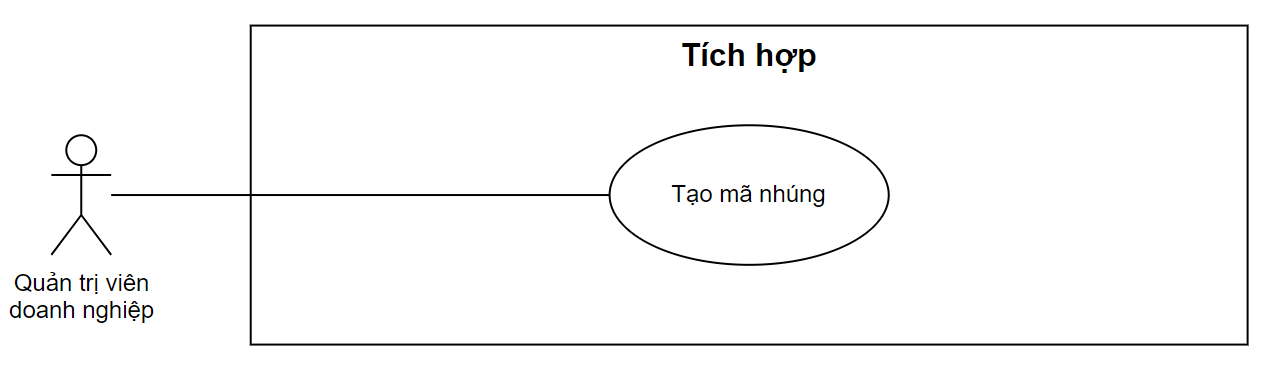
\includegraphics[width=1\linewidth]{Dg_UC/tichhop.png}
    \vspace{0.5cm}
    \caption{Biểu đồ use case cho tích hợp}
    \label{fig:enter-label}
\end{figure}
\subsubsubsection{Usecase scenerio}
\textbf{Tạo mã nhúng}

\begin{table}[H]
\centering
\begin{tabular}{|l|l|l|l|}
\hline
Use case name: & \multicolumn{3}{|l|}{Tạo mã nhúng} \\
\hline
Created by: & Phạm Đức Thắng & Last updated by: & Phạm Đức Thắng \\
\hline
Date created: & 19/10/2024 & Date last updated: & 19/10/2024 \\
\hline
Actors: & \multicolumn{3}{|l|}{Quản trị viên doanh nghiệp} \\
\hline
Description: & \multicolumn{3}{|p{12cm}|}{Quản trị viên doanh nghiệp tạo đoạn mã nhúng và gắn vào website để có thể tích hợp chatbot vào website của họ.} \\
\hline
Trigger: & \multicolumn{3}{|p{12cm}|}{Quản trị viên muốn tạo mã nhúng để tích hợp chatbot vào website.} \\
\hline
Preconditions: & \multicolumn{3}{|p{12cm}|}{
- Quản trị viên đã đăng nhập vào hệ thống. \newline
- Doanh nghiệp đã đăng ký dịch vụ chatbot.
} \\
\hline
Postconditions: & \multicolumn{3}{|p{12cm}|}{Đoạn mã nhúng được tạo thành công và sẵn sàng để tích hợp.} \\
\hline
Normal Flows: & \multicolumn{3}{|p{12cm}|}{
1. Quản trị viên đăng nhập vào hệ thống quản lý chatbot. \newline
2. Điều hướng tới trang “Tùy chỉnh chatbot”. \newline
3. Xem trước kích thước, màu sắc, vị trí hiển thị của chatbot. \newline
4. Nhấn nút "Tạo mã nhúng". \newline
5. Hệ thống tạo và hiển thị đoạn mã nhúng. \newline
6. Quản trị viên sao chép đoạn mã này để gán vào website.
}\\
\hline
Alternative Flows: & \multicolumn{3}{|p{12cm}|}{Không có} \\
\hline
Exceptions: & \multicolumn{3}{|p{12cm}|}{
\textbf{E1: Xảy ra sự cố kỹ thuật trong quá trình tạo đoạn mã nhúng} \newline
5.1. Hệ thống hiển thị thông báo lỗi: "Đã xảy ra lỗi trong quá trình tạo đoạn mã nhúng. Vui lòng thử lại sau."
} \\
\hline
Notes and issues: & \multicolumn{3}{|p{12cm}|}{Không có} \\
\hline
\end{tabular}
\caption{Use case scenario cho Tạo mã nhúng}
\end{table}

%-------------------------------------------------------------------
\subsubsection{Quản lý chatbot}
\subsubsubsection{Biểu đồ use case}
\begin{figure}[H]
    \centering
    % 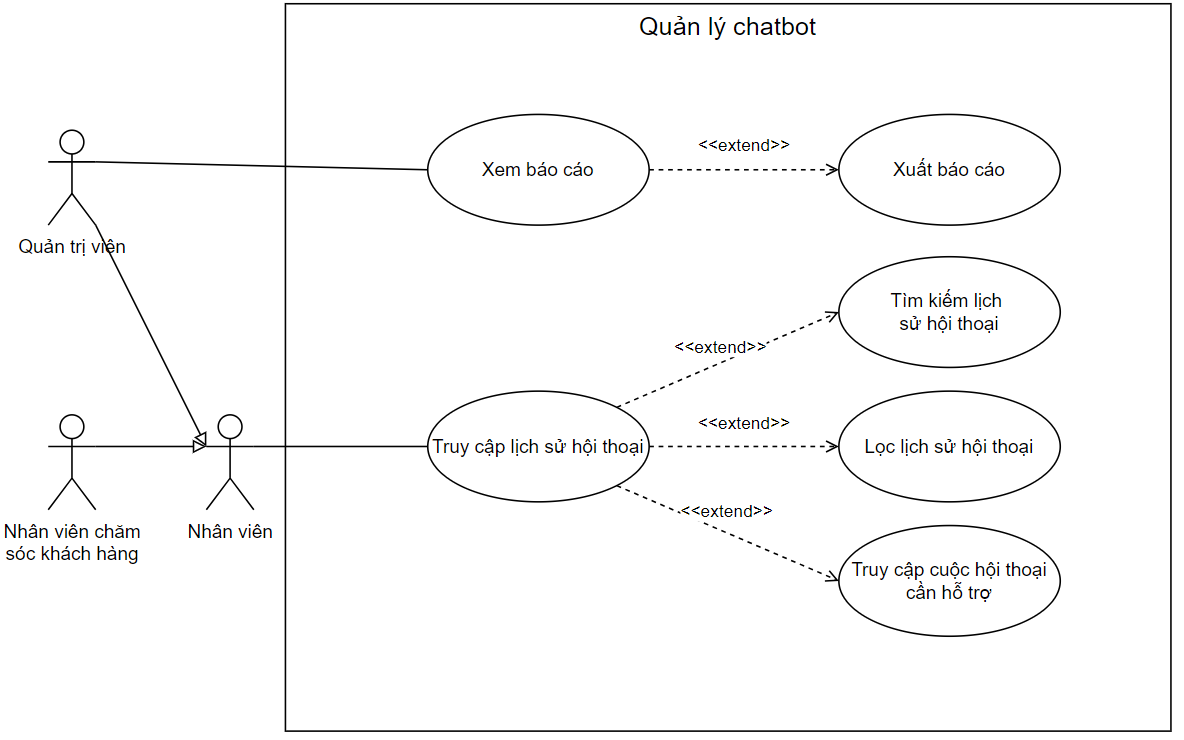
\includegraphics[width=1\linewidth]{Dg_UC/quanlychatbot.png}
    \includesvg[width=1\textwidth]{Dg_UC/Usecase Diagram-ChatbotManagement.drawio.svg}
    \vspace{0.5cm}
    \caption{Biểu đồ use case cho Quản lý chatbot}
    \label{fig:enter-label}
\end{figure}
\subsubsubsection{Use case scenario}
\textbf{Xem báo cáo}
\begin{table}[H]
    \centering
    \begin{tabular}{|l|l|l|l|} 
        \hline
        Use case name: & \multicolumn{3}{|l|}{Xem báo cáo} \\
        \hline
        Created by: & Lê Đình Huy & Last updated by: & Lê Đình Huy \\
        \hline
        Date created: & 19 / 10 / 2024 & Date last updated: & 19 / 10 / 2024 \\
        \hline
        Actors: & \multicolumn{3}{|l|}{Quản trị viên} \\
        \hline
        Description: & \multicolumn{3}{|p{12cm}|}{Cho phép quản trị viên xem báo cáo thống kê về hệ thống chatbot của mình.} \\ 
        \hline
        Trigger: & \multicolumn{3}{|p{12cm}|}{Chọn "Báo cáo" trên thanh điều hướng.} \\
        \hline
        Preconditions: & \multicolumn{3}{|p{12cm}|}{- Quản trị viên có tài khoản trên website. \newline
        - Quản trị viên đã đăng nhập thành công vào hệ thống. \newline
        - Thiết bị của quản trị viên có kết nối mạng và kết nối với hệ thống. \newline
        - Quản trị viên có quyền thực hiện chức năng.} \\
        \hline
        Postconditions: & \multicolumn{3}{|p{12cm}|}{Hệ thống hiển thị các thông số và biểu đồ thống kê.} \\
        \hline
        Normal Flows: & \multicolumn{3}{|p{12cm}|}{1. Quản trị viên chọn "Báo cáo" trên thanh điều hướng. \newline
        2. Hệ thống hiển thị các thông số và báo cáo thống kê.}\\
        \hline
        Alternative Flows: & \multicolumn{3}{|p{12cm}|}{\textbf{A1: Sau bước 2} \newline
        3.1. Quản trị viên chọn "Lọc".\newline
        3.2. Hệ thống hiển thị các thông số cho phép của bộ lọc.\newline
        3.3. Quản trị viên chọn một thông số.\newline
        Tiếp tục bước 2 trong Normal flows.
        } \\
        \hline
        Exceptions: & \multicolumn{3}{|p{12cm}|}{Không có} \\
        \hline
        Note and issues: & \multicolumn{3}{|p{12cm}|}{Không có} \\
        \hline
    \end{tabular}
    \caption{Use case scenario cho Xem báo cáo}
\end{table}

\textbf{Xuất báo cáo}
\begin{table}[H]
    \centering
    \begin{tabular}{|l|l|l|l|} 
        \hline
        Use case name: & \multicolumn{3}{|l|}{Xuất báo cáo} \\
        \hline
        Created by: & Lê Đình Huy & Last updated by: & Lê Đình Huy \\
        \hline
        Date created: & 19 / 10 / 2024 & Date last updated: & 19 / 10 / 2024 \\
        \hline
        Actors: & \multicolumn{3}{|l|}{Quản trị viên} \\
        \hline
        Description: & \multicolumn{3}{|p{12cm}|}{Cho phép quản trị viên xuất báo cáo thống kê về hệ thống chatbot của mình ra file pdf hoặc excel.} \\ 
        \hline
        Trigger: & \multicolumn{3}{|p{12cm}|}{Chọn "Xuất báo cáo" trong giao diện Xem báo cáo.} \\
        \hline
        Preconditions: & \multicolumn{3}{|p{12cm}|}{- Quản trị viên có tài khoản trên website. \newline
        - Quản trị viên đã đăng nhập thành công vào hệ thống. \newline
        - Thiết bị của quản trị viên có kết nối mạng và kết nối với hệ thống. \newline
        - Quản trị viên có quyền thực hiện chức năng.} \\
        \hline
        Postconditions: & \multicolumn{3}{|p{12cm}|}{File báo cáo được tạo và tải về thiết bị của quản trị viên.} \\
        \hline
        Normal Flows: & \multicolumn{3}{|p{12cm}|}{1. Quản trị viên chọn "Xuất báo cáo" trong giao diện Xem báo cáo.\newline
        2. Hệ thống hiển thị hai loại tệp (pdf, excel) cho quản trị viên chọn.\newline
        3. Quản trị viên chọn một loại tệp và chọn "Xem trước".\newline
        4. Hệ thống hiển thị chế độ xem trước file.\newline
        5. Quản trị viên chọn "Tải xuống". \newline
        6. File báo cáo được tải về thiết bị của quản trị viên.}\\
        \hline
        Alternative Flows: & \multicolumn{3}{|p{12cm}|}{Không có} \\
        \hline
        Exceptions: & \multicolumn{3}{|p{12cm}|}{
        \textbf{E1: Tại bước 5} \newline
        5.1. Quản trị viên chọn "Hủy bỏ".\newline
        5.2. Hệ thống đóng chế độ xem trước file.\newline
        Use case dừng lại.
        } \\
        \hline
        Note and issues: & \multicolumn{3}{|p{12cm}|}{Không có} \\
        \hline
    \end{tabular}
    \caption{Use case scenario cho Xem báo cáo}
\end{table}

\textbf{Truy cập lịch sử hội thoại}
\begin{table}[H]
    \centering
    \begin{tabular}{|l|l|l|l|} 
        \hline
        Use case name: & \multicolumn{3}{|l|}{Truy cập lịch sử hội thoại} \\
        \hline
        Created by: & Lê Đình Huy & Last updated by: & Lê Đình Huy \\
        \hline
        Date created: & 19 / 10 / 2024 & Date last updated: & 19 / 10 / 2024 \\
        \hline
        Actors: & \multicolumn{3}{|l|}{Nhân viên} \\
        \hline
        Description: & \multicolumn{3}{|p{12cm}|}{Cho phép nhân viên truy cập và xem lịch sử hội thoại.} \\ 
        \hline
        Trigger: & \multicolumn{3}{|p{12cm}|}{Chọn "Chat" trên thanh điều hướng.} \\
        \hline
        Preconditions: & \multicolumn{3}{|p{12cm}|}{- Nhân viên có tài khoản trên website. \newline
        - Nhân viên đã đăng nhập thành công vào hệ thống. \newline
        - Thiết bị của nhân viên có kết nối mạng và kết nối với hệ thống. \newline
        - Nhân viên có quyền thực hiện chức năng.} \\
        \hline
        Postconditions: & \multicolumn{3}{|p{12cm}|}{Hệ thống hiển thị chi tiết toàn bộ cuộc hội thoại của khách hàng.} \\
        \hline
        Normal Flows: & \multicolumn{3}{|p{12cm}|}{1. Nhân viên chọn "Chat" trên thanh điều hướng.\newline
        2. Hệ thống hiển thị danh sách các cuộc hội thoại.\newline
        3. Nhân viên chọn xem một cuộc hội thoại.\newline
        4. Hệ thống hiển thị chi tiết toàn bộ cuộc hội thoại của khách hàng.}\\
        \hline
        Alternative Flows: & \multicolumn{3}{|p{12cm}|}{
        \textbf{A1: Tại bước 3}\newline
        3.1. Nhân viên chọn vào ô Tìm kiếm và nhập nội dung cần tìm.\newline
        3.2. Nhân viên chọn "Tìm".\newline
        Tiếp tục bước 2 trong Normal flows.\newline
        \textbf{A2: Tại bước 3}\newline
        3.1. Nhân viên chọn "Lọc".\newline
        3.2. Hệ thống hiển thị các thông số cho phép của bộ lọc.\newline
        3.3. Nhân viên chọn một thông số.\newline
        Tiếp tục bước 2 trong Normal flows.\newline
        \textbf{A3: Tại bước 3}\newline
        3.1. Nhân viên chọn "Cần hỗ trợ".\newline
        Tiếp tục bước 2 trong Normal flows.
        } \\
        \hline
        Exceptions: & \multicolumn{3}{|p{12cm}|}{Không có} \\
        \hline
        Note and issues: & \multicolumn{3}{|p{12cm}|}{Không có} \\
        \hline
    \end{tabular}
    \caption{Use case scenario cho Xem báo cáo}
\end{table}

%-------------------------------------------------------------------
\subsubsection{Thông báo và cảnh báo}
\subsubsubsection{Biểu đồ use case}
\begin{figure}[H]
    \centering
    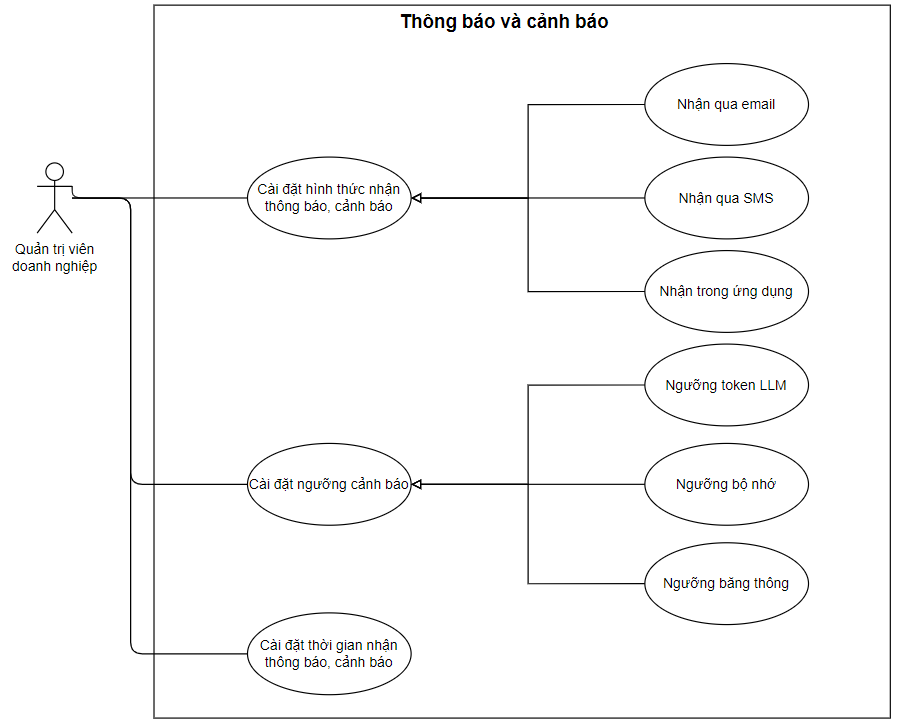
\includegraphics[width=1\linewidth]{Dg_UC/thongbaocanhbao.png}
    \vspace{0.5cm}
    \caption{Biểu đồ use case cho Thông báo và cảnh báo}
    \label{fig:enter-label}
\end{figure}
\subsubsubsection{Use case scenario}

\textbf{Chọn phương thức thông báo và cảnh báo}
\begin{table}[H]
\centering
\begin{tabular}{|l|l|l|l|}
\hline
Use case name: & \multicolumn{3}{|l|}{Chọn phương thức thông báo và cảnh báo} \\
\hline
Created by: & Phạm Đức Thắng & Last updated by: & Phạm Đức Thắng \\
\hline
Date created: & 19/10/2024 & Date last updated: & 19/10/2024 \\
\hline
Actors: & \multicolumn{3}{|l|}{Quản trị viên doanh nghiệp} \\
\hline
Description: & \multicolumn{3}{|p{12cm}|}{Doanh nghiệp có thể chọn cách họ muốn nhận thông báo và cảnh báo liên quan đến hệ thống chatbot.} \\
\hline
Trigger: & \multicolumn{3}{|p{12cm}|}{Quản trị viên muốn thay đổi phương thức nhận thông báo và cảnh báo.} \\
\hline
Preconditions: & \multicolumn{3}{|p{12cm}|}{Người dùng đã đăng nhập vào hệ thống.} \\
\hline
Postconditions: & \multicolumn{3}{|p{12cm}|}{Phương thức thông báo và cảnh báo được lưu và áp dụng cho tài khoản doanh nghiệp.} \\
\hline
Normal Flows: & \multicolumn{3}{|p{12cm}|}{
1. Người dùng truy cập vào trang cài đặt thông báo và cảnh báo. \newline
2. Hệ thống hiển thị các tùy chọn phương thức. \newline
3. Người dùng chọn hoặc hủy chọn các phương thức nhận thông báo: email và trong ứng dụng. \newline
4. Người dùng xác nhận lựa chọn. \newline
5. Hệ thống lưu cài đặt và hiển thị thông báo xác nhận.
}\\
\hline
Alternative Flows: & \multicolumn{3}{|p{12cm}|}{Không có} \\
\hline
Exceptions: & \multicolumn{3}{|p{12cm}|}{
\textbf{E1. Hệ thống không thể lưu cài đặt} \newline
5.1. Hệ thống hiển thị thông báo lỗi. \newline
5.2. Người dùng có thể thử lại hoặc hủy bỏ thao tác.
} \\
\hline
Notes and issues: & \multicolumn{3}{|p{12cm}|}{Không có} \\
\hline
\end{tabular}
\caption{Use case scenario cho Chọn phương thức thông báo và cảnh báo}
\end{table}

\textbf{Thiết lập ngưỡng cảnh báo}

\begin{table}[H]
\centering
\begin{tabular}{|l|l|l|l|}
\hline
Use case name: & \multicolumn{3}{|l|}{Thiết lập ngưỡng cảnh báo} \\
\hline
Created by: & Phạm Đức Thắng & Last updated by: & Phạm Đức Thắng \\
\hline
Date created: & 19/10/2024 & Date last updated: & 19/10/2024 \\
\hline
Actors: & \multicolumn{3}{|l|}{Quản trị viên doanh nghiệp} \\
\hline
Description: & \multicolumn{3}{|p{12cm}|}{Doanh nghiệp có thể thiết lập ngưỡng cảnh báo cho việc sử dụng token LLM và lưu lượng truy cập.} \\
\hline
Trigger: & \multicolumn{3}{|p{12cm}|}{Quản trị viên muốn thay đổi ngưỡng cảnh báo cho việc sử dụng token LLM và lưu lượng truy cập.} \\
\hline
Preconditions: & \multicolumn{3}{|p{12cm}|}{Người dùng đã đăng nhập vào hệ thống.} \\
\hline
Postconditions: & \multicolumn{3}{|p{12cm}|}{Ngưỡng cảnh báo được lưu và áp dụng cho tài khoản người dùng.} \\
\hline
Normal Flows: & \multicolumn{3}{|p{12cm}|}{
1. Người dùng truy cập vào trang cài đặt thông báo và cảnh báo. \newline
2. Hệ thống hiển thị các tùy chọn ngưỡng. \newline
3. Người dùng thiết lập ngưỡng cảnh báo cho việc sử dụng token LLM. \newline
4. Người dùng thiết lập ngưỡng cảnh báo cho lưu lượng truy cập. \newline
5. Người dùng xác nhận các cài đặt. \newline
6. Hệ thống lưu cài đặt và hiển thị thông báo xác nhận.
}\\
\hline
Alternative Flows: & \multicolumn{3}{|p{12cm}|}{
\textbf{A1. Người dùng tắt cảnh báo cho việc sử dụng token LLM} \newline
3.1. Người dùng bấm nút tắt cảnh báo cho việc sử dụng token LLM \newline
\textbf{A2. Người dùng tắt cảnh báo cho lưu lượng truy cập} \newline
4.1. Người dùng bấm nút tắt cảnh báo cho lưu lượng truy cập
} \\
\hline
Exceptions: & \multicolumn{3}{|p{12cm}|}{
\textbf{E1. Hệ thống không thể lưu cài đặt} \newline
6.1. Hệ thống hiển thị thông báo lỗi. \newline
6.2. Người dùng có thể thử lại hoặc hủy bỏ thao tác.
} \\
\hline
Notes and issues: & \multicolumn{3}{|p{12cm}|}{Không có} \\
\hline
\end{tabular}
\caption{Use case scenario cho Thiết lập ngưỡng cảnh báo}
\end{table}

%-------------------------------------------------------------------
\subsubsection{Quản lý thanh toán}
\subsubsubsection{Biểu đồ usecase}
\begin{figure}[H]
    \centering
    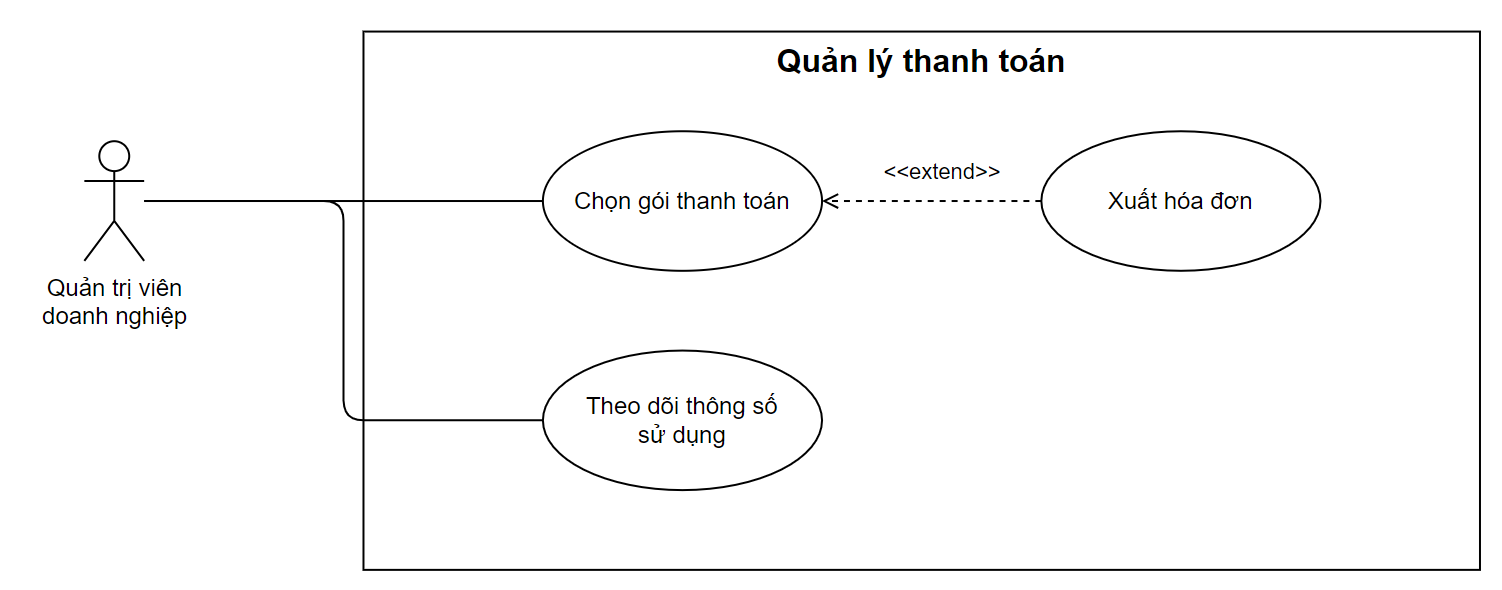
\includegraphics[width=1\linewidth]{Dg_UC/quanlythanhtoan.png}
    \vspace{0.5cm}
    \caption{Biểu đồ use case cho Quản lý thanh toán}
    \label{fig:enter-label}
\end{figure}
\subsubsubsection{Usecase scenerio}
\textbf{Chọn gói thanh toán}

\begin{table}[H]
\centering
\begin{tabular}{|l|l|l|l|}
\hline
Use case name: & \multicolumn{3}{|l|}{Chọn gói thanh toán} \\
\hline
Created by: & Phạm Đức Thắng & Last updated by: & Phạm Đức Thắng \\
\hline
Date created: & 19/10/2024 & Date last updated: & 19/10/2024 \\
\hline
Actors: & \multicolumn{3}{|l|}{Doanh nghiệp} \\
\hline
Description: & \multicolumn{3}{|p{12cm}|}{Doanh nghiệp lựa chọn gói đăng ký phù hợp với nhu cầu sử dụng dịch vụ chatbot từ các gói có sẵn trên hệ thống.} \\
\hline
Trigger: & \multicolumn{3}{|p{12cm}|}{Doanh nghiệp muốn chọn hoặc thay đổi gói đăng ký dịch vụ chatbot.} \\
\hline
Preconditions: & \multicolumn{3}{|p{12cm}|}{
- Doanh nghiệp đã đăng ký và đăng nhập vào tài khoản của mình trên hệ thống. \newline
- Hệ thống đã có các gói đăng ký được cấu hình sẵn.
} \\
\hline
Postconditions: & \multicolumn{3}{|p{12cm}|}{
- Doanh nghiệp đã chọn và xác nhận gói đăng ký mới. \newline
- Hệ thống đã cập nhật gói đăng ký của doanh nghiệp và thực hiện thanh toán nếu cần.
} \\
\hline
Normal Flows: & \multicolumn{3}{|p{12cm}|}{
1. Doanh nghiệp đăng nhập vào tài khoản của mình trên trang web hoặc ứng dụng. \newline
2. Doanh nghiệp điều hướng vào trang "Gói đăng ký". \newline
3. Hệ thống hiển thị danh sách các gói đăng ký hiện có với các tính năng và giá cả tương ứng. \newline
4. Doanh nghiệp chọn gói đăng ký mong muốn bằng cách nhấp vào nút "Mua". \newline
5. Hệ thống hiển thị thông tin chi tiết của gói đăng ký đã chọn và yêu cầu xác nhận. \newline
6. Doanh nghiệp xác nhận lựa chọn và tiến hành thanh toán. \newline
7. Hệ thống xử lý giao dịch thanh toán và cập nhật trạng thái gói đăng ký cho doanh nghiệp. \newline
8. Hệ thống hiển thị thông báo xác nhận thành công.
}\\
\hline
Alternative Flows: & \multicolumn{3}{|p{12cm}|}{
\textbf{A1: Thay đổi gói đăng ký} \newline
4.1. Doanh nghiệp chọn gói đăng ký mới muốn nâng cấp hoặc giảm cấp. \newline
4.2. Hệ thống tính toán sự khác biệt về giá cả hoặc phí áp dụng nếu có. \newline
4.3. Doanh nghiệp xác nhận lựa chọn và tiến hành thanh toán nếu cần. \newline
4.4. Hệ thống cập nhật gói đăng ký mới cho doanh nghiệp và điều chỉnh các dịch vụ liên quan. \newline\newline
\textbf{A2: Doanh nghiệp chọn xuất hóa đơn} \newline
6.1. Sau khi thanh toán thành công, hệ thống cung cấp tùy chọn "Xuất Hóa Đơn". \newline
6.2. Doanh nghiệp chọn "Xuất Hóa Đơn" để tải xuống hóa đơn hoặc gửi qua email. \newline
6.3. Hệ thống tạo và gửi hóa đơn đến email đã đăng ký. \newline
6.4. Doanh nghiệp nhận được hóa đơn để lưu trữ và quản lý chi tiêu.
} \\
\hline
Exceptions: & \multicolumn{3}{|p{12cm}|}{
\textbf{E1 Giao dịch thanh toán không thành công do lỗi thẻ tín dụng, thiếu tiền trong tài khoản hoặc sự cố mạng.} \newline
7.1. Khi doanh nghiệp cố gắng thanh toán, hệ thống kiểm tra và phát hiện lỗi. \newline
7.2. Hệ thống hiển thị thông báo lỗi: "Thanh toán không thành công. Vui lòng kiểm tra thông tin thanh toán hoặc thử lại sau." \newline
7.3. Doanh nghiệp có thể thử lại giao dịch hoặc thay đổi thông tin thanh toán khác.
} \\
\hline
Notes and issues: & \multicolumn{3}{|p{12cm}|}{Không có} \\
\hline
\end{tabular}
\caption{Use case scenario cho Chọn gói thanh toán}
\end{table}

\textbf{Theo dõi thông số sử dụng}

\begin{table}[H]
\centering
\begin{tabular}{|l|l|l|l|}
\hline
Use case name: & \multicolumn{3}{|l|}{Theo dõi thông số sử dụng} \\
\hline
Created by: & Phạm Đức Thắng & Last updated by: & Phạm Đức Thắng \\
\hline
Date created: & 19/10/2024 & Date last updated: & 19/10/2024 \\
\hline
Actors: & \multicolumn{3}{|l|}{Doanh nghiệp} \\
\hline
Description: & \multicolumn{3}{|p{12cm}|}{Doanh nghiệp có thể theo dõi các thông số giới han của gói đã đăng ký, bao gồm thời hạn gói đăng ký, số lượng yêu cầu và bộ nhớ đã sử dụng.} \\
\hline
Trigger: & \multicolumn{3}{|p{12cm}|}{Doanh nghiệp muốn xem thông tin về mức độ sử dụng dịch vụ chatbot.} \\
\hline
Preconditions: & \multicolumn{3}{|p{12cm}|}{
- Doanh nghiệp đã đăng ký và sử dụng dịch vụ chatbot. \newline
- Hệ thống đã ghi nhận dữ liệu sử dụng dịch vụ của doanh nghiệp.
} \\
\hline
Postconditions: & \multicolumn{3}{|p{12cm}|}{Doanh nghiệp đã xem được các thông số sử dụng dịch vụ chi tiết.} \\
\hline
Normal Flows: & \multicolumn{3}{|p{12cm}|}{
1. Doanh nghiệp đăng nhập vào tài khoản của mình. \newline
2. Doanh nghiệp truy cập vào trang "Quản lý thanh toán". \newline
3. Hệ thống hiển thị các thông số sử dụng hiện tại như số lượng yêu cầu đã xử lý, thời gian gói còn lại và bộ nhớ đã sử dụng.
}\\
\hline
Alternative Flows: & \multicolumn{3}{|p{12cm}|}{Không có} \\
\hline
Exceptions: & \multicolumn{3}{|p{12cm}|}{
\textbf{E1: Hệ thống chưa có dữ liệu sử dụng do mới bắt đầu dịch vụ hoặc vấn đề kỹ thuật} \newline
5.1. Hệ thống kiểm tra và phát hiện thiếu dữ liệu. \newline
5.2. Hiển thị thông báo: "Chưa có dữ liệu sử dụng để hiển thị. Vui lòng quay lại sau."
} \\
\hline
Notes and issues: & \multicolumn{3}{|p{12cm}|}{Không có} \\
\hline
\end{tabular}
\caption{Use case scenario cho Theo dõi sử dụng}
\end{table}

%-------------------------------------------------------------------
\subsubsection{Tương tác với chatbot}
\subsubsubsection{Biểu đồ use case}
\begin{figure}[H]
    \centering
    % 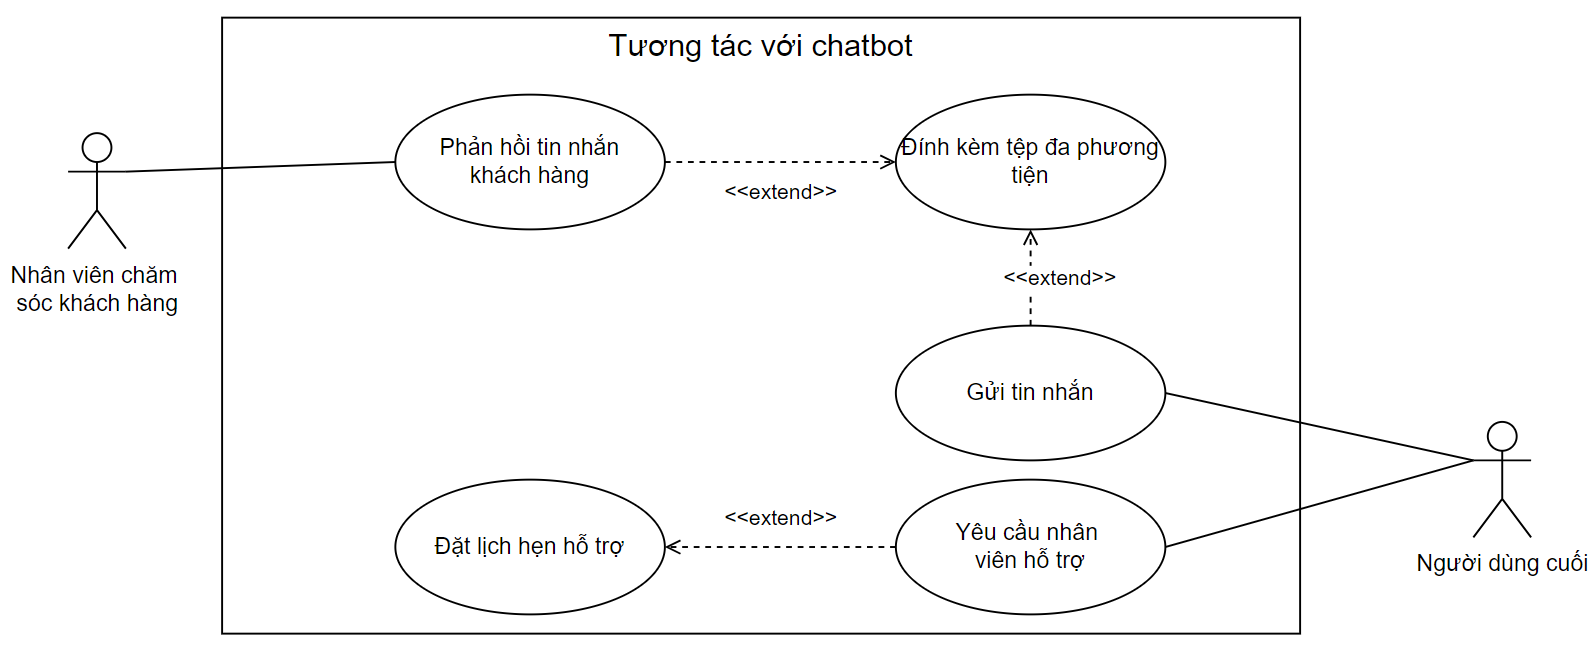
\includegraphics[width=1\linewidth]{Dg_UC/tuongtacvoichatbot.png}
    \includesvg[width=1\textwidth]{Dg_UC/Usecase Diagram-ChatbotInteraction.drawio.svg}
    \vspace{0.5cm}
    \caption{Biểu đồ use case cho Tương tác với chatbot}
    \label{fig:enter-label}
\end{figure}
\subsubsubsection{Use case scenario}
\textbf{Phản hồi tin nhắn khách hàng}
\begin{table}[H]
    \centering
    \begin{tabular}{|l|l|l|l|} 
        \hline
        Use case name: & \multicolumn{3}{|l|}{Phản hồi tin nhắn khách hàng} \\
        \hline
        Created by: & Lê Đình Huy & Last updated by: & Lê Đình Huy \\
        \hline
        Date created: & 19 / 10 / 2024 & Date last updated: & 19 / 10 / 2024 \\
        \hline
        Actors: & \multicolumn{3}{|l|}{Nhân viên chăm sóc khách hàng} \\
        \hline
        Description: & \multicolumn{3}{|p{12cm}|}{Cho phép nhân viên chăm sóc khách hàng phản hồi trực tiếp tin nhắn của khách hàng.} \\ 
        \hline
        Trigger: & \multicolumn{3}{|p{12cm}|}{Chọn vào xem đoạn hội thoại với một khách hàng.} \\
        \hline
        Preconditions: & \multicolumn{3}{|p{12cm}|}{- Nhân viên có tài khoản trên website. \newline
        - Nhân viên đã đăng nhập thành công vào hệ thống. \newline
        - Thiết bị của nhân viên có kết nối mạng và kết nối với hệ thống. \newline
        - Nhân viên có quyền thực hiện chức năng.} \\
        \hline
        Postconditions: & \multicolumn{3}{|p{12cm}|}{Tin nhắn được gửi thành công và hiển thị ở hai phía.} \\
        \hline
        Normal Flows: & \multicolumn{3}{|p{12cm}|}{1. Nhân viên CSKH chọn vào xem đoạn hội thoại với một khách hàng. \newline
        2. Hệ thống hiển thị màn hình chat với khách hàng đó. \newline
        3. Nhân viên CSKH chọn vào khung điền tin nhắn và nhập nội dung tin nhắn. \newline
        4. Nhân viên CSKH chọn "Gửi". \newline
        5. Hệ thống lưu dữ liệu vào database và hiển thị tin nhắn vừa gửi lên màn hình.} \\
        \hline
        Alternative Flows: & \multicolumn{3}{|p{12cm}|}{\textbf{A1: Tại bước 3 hoặc 4} \newline
        Khi nhân viên CSKH muốn đính kèm tệp, chuyển đến use case Đính kèm tệp đa phương tiện. Sau đó tiếp tục tại bước đó trong Normal flows.} \\
        \hline
        Exceptions: & \multicolumn{3}{|p{12cm}|}{Không có} \\
        \hline
        Note and issues: & \multicolumn{3}{|p{12cm}|}{Không có} \\
        \hline
    \end{tabular}
    \caption{Use case scenario cho Phản hồi tin nhắn khách hàng}
\end{table}

\textbf{Gửi tin nhắn}
\begin{table}[H]
    \centering
    \begin{tabular}{|l|l|l|l|} 
        \hline
        Use case name: & \multicolumn{3}{|l|}{Gửi tin nhắn} \\
        \hline
        Created by: & Lê Đình Huy & Last updated by: & Lê Đình Huy \\
        \hline
        Date created: & 19 / 10 / 2024 & Date last updated: & 19 / 10 / 2024 \\
        \hline
        Actors: & \multicolumn{3}{|l|}{Người dùng cuối (Khách hàng)} \\
        \hline
        Description: & \multicolumn{3}{|p{12cm}|}{Cho phép người dùng cuối gửi tin nhắn trong chatbot.} \\ 
        \hline
        Trigger: & \multicolumn{3}{|p{12cm}|}{Chọn vào nút chatbot trên website của doanh nghiệp.} \\
        \hline
        Preconditions: & \multicolumn{3}{|p{12cm}|}{- Thiết bị của người dùng có kết nối mạng.} \\
        \hline
        Postconditions: & \multicolumn{3}{|p{12cm}|}{Tin nhắn được gửi thành công và hiển thị trên màn hình. \newline
        Đồng thời, tin nhắn từ chatbot sẽ phản hồi lại trong một khoảng thời gian nhất định.} \\
        \hline
        Normal Flows: & \multicolumn{3}{|p{12cm}|}{1. Người dùng chọn vào nút chatbot trên website của doanh nghiệp. \newline
        2. Hệ thống hiển thị màn hình chatbot. \newline
        3. Người dùng chọn vào khung điền tin nhắn và nhập nội dung tin nhắn. \newline
        4. Người dùng chọn "Gửi". \newline
        5. Hệ thống lưu dữ liệu vào database và hiển thị tin nhắn vừa gửi lên màn hình. \newline
        6. Hệ thống chatbot tạo và phản hồi người dùng trong một khoảng thời gian nhất định.} \\
        \hline
        Alternative Flows: & \multicolumn{3}{|p{12cm}|}{\textbf{A1: Tại bước 3 hoặc 4} \newline
        Khi người dùng muốn đính kèm tệp, chuyển đến use case Đính kèm tệp đa phương tiện. Sau đó tiếp tục tại bước đó trong Normal flows.} \\
        \hline
        Exceptions: & \multicolumn{3}{|p{12cm}|}{Không có} \\
        \hline
        Note and issues: & \multicolumn{3}{|p{12cm}|}{Không có} \\
        \hline
    \end{tabular}
    \caption{Use case scenario cho Gửi tin nhắn}
\end{table}


\textbf{Đính kèm tệp đa phương tiện}
\begin{table}[H]
    \centering
    \begin{tabular}{|l|l|l|l|} 
        \hline
        Use case name: & \multicolumn{3}{|l|}{Đính kèm tệp đa phương tiện} \\
        \hline
        Created by: & Lê Đình Huy & Last updated by: & Lê Đình Huy \\
        \hline
        Date created: & 19 / 10 / 2024 & Date last updated: & 19 / 10 / 2024 \\
        \hline
        Actors: & \multicolumn{3}{|l|}{Nhân viên CSKH, người dùng cuối (Khách hàng)} \\
        \hline
        Description: & \multicolumn{3}{|p{12cm}|}{Cho phép nhân viên CSKH và người dùng cuối đính kèm tệp đa phương tiện.} \\ 
        \hline
        Trigger: & \multicolumn{3}{|p{12cm}|}{Chọn vào nút "Đính kèm tệp đa phương tiện" trong khung chat.} \\
        \hline
        Preconditions: & \multicolumn{3}{|p{12cm}|}{Preconditions của tính năng Phản hồi tin nhắn khách hàng đối với nhân viên CSKH, tính năng Gửi tin nhắn đối với người dùng cuối.} \\
        \hline
        Postconditions: & \multicolumn{3}{|p{12cm}|}{Hệ thống hiển thị ảnh được chọn lên màn hình.} \\
        \hline
        Normal Flows: & \multicolumn{3}{|p{12cm}|}{1. Người dùng chọn vào nút "Đính kèm tệp đa phương tiện". \newline
        2. Hệ thống hiển thị màn hình chọn ảnh. \newline
        3. Người dùng chọn một bức ảnh trên thiết bị. \newline
        4. Người dùng chọn "Tải lên". \newline
        5. Hệ thống hiển thị ảnh được chọn lên màn hình.} \\
        \hline
        Alternative Flows: & \multicolumn{3}{|p{12cm}|}{Không có} \\
        \hline
        Exceptions: & \multicolumn{3}{|p{12cm}|}{\textbf{E1: Sau bước 5} \newline
        6.1. Người dùng chọn nút "Xóa" ảnh vừa tải. \newline
        6.2. Ảnh vừa tải bị xóa khỏi màn hình. \newline
        Use case dừng lại.} \\
        \hline
        Note and issues: & \multicolumn{3}{|p{12cm}|}{Không có} \\
        \hline
    \end{tabular}
    \caption{Use case scenario cho Đính kèm tệp đa phương tiện}
\end{table}


\textbf{Yêu cầu nhân viên hỗ trợ}
\begin{table}[H]
    \centering
    \begin{tabular}{|l|l|l|l|} 
        \hline
        Use case name: & \multicolumn{3}{|l|}{Yêu cầu nhân viên hỗ trợ} \\
        \hline
        Created by: & Lê Đình Huy & Last updated by: & Lê Đình Huy \\
        \hline
        Date created: & 19 / 10 / 2024 & Date last updated: & 19 / 10 / 2024 \\
        \hline
        Actors: & \multicolumn{3}{|l|}{Người dùng cuối (Khách hàng)} \\
        \hline
        Description: & \multicolumn{3}{|p{12cm}|}{Cho phép người dùng cuối có thể yêu cầu nhân viên hỗ trợ.} \\ 
        \hline
        Trigger: & \multicolumn{3}{|p{12cm}|}{Chọn vào nút yêu cầu hỗ trợ trong khung chatbot.} \\
        \hline
        Preconditions: & \multicolumn{3}{|p{12cm}|}{- Thiết bị của người dùng có kết nối mạng.} \\
        \hline
        Postconditions: & \multicolumn{3}{|p{12cm}|}{Yêu cầu được gửi lên hệ thống và màn hình hiển thị thông báo thành công. Đồng thời, tính năng chat tự động sẽ được tạm dừng.} \\
        \hline
        Normal Flows: & \multicolumn{3}{|p{12cm}|}{1. Người dùng chọn vào nút yêu cầu hỗ trợ trong khung chatbot. \newline
        2. Hệ thống hiển thị pop up Hỗ trợ khách hàng. \newline
        3. Người dùng chọn "Gửi yêu cầu". \newline
        4. Yêu cầu được gửi lên hệ thống và màn hình hiển thị thông báo thành công. Đồng thời, tính năng chat tự động sẽ được tạm dừng.} \\
        \hline
        Alternative Flows: & \multicolumn{3}{|p{12cm}|}{Không có} \\
        \hline
        Exceptions: & \multicolumn{3}{|p{12cm}|}{\textbf{E1: Tại bước 3} \newline
        3.1. Người dùng chọn "Đặt lịch hẹn". \newline
        Chuyển đến use case Đặt lịch hẹn hỗ trợ. Use case dừng lại. \newline
        \textbf{E2: Tại bước 3} \newline
        3.1. Người dùng chọn "Đóng". \newline
        3.2. Pop up Hỗ trợ khách hàng được đóng. \newline
        Use case dừng lại.} \\
        \hline
        Note and issues: & \multicolumn{3}{|p{12cm}|}{Không có} \\
        \hline
    \end{tabular}
    \caption{Use case scenario cho Yêu cầu nhân viên hỗ trợ}
\end{table}


\textbf{Đặt lịch hẹn hỗ trợ}
\begin{table}[H]
    \centering
    \begin{tabular}{|l|l|l|l|} 
        \hline
        Use case name: & \multicolumn{3}{|l|}{Đặt lịch hẹn hỗ trợ} \\
        \hline
        Created by: & Lê Đình Huy & Last updated by: & Lê Đình Huy \\
        \hline
        Date created: & 19 / 10 / 2024 & Date last updated: & 19 / 10 / 2024 \\
        \hline
        Actors: & \multicolumn{3}{|l|}{Người dùng cuối (Khách hàng)} \\
        \hline
        Description: & \multicolumn{3}{|p{12cm}|}{Cho phép người dùng cuối có thể đặt lịch hẹn hỗ trợ theo thời gian mình mong muốn.} \\ 
        \hline
        Trigger: & \multicolumn{3}{|p{12cm}|}{Chọn vào nút "Đặt lịch hẹn" trong pop up Hỗ trợ khách hàng.} \\
        \hline
        Preconditions: & \multicolumn{3}{|p{12cm}|}{- Thiết bị của người dùng có kết nối mạng.} \\
        \hline
        Postconditions: & \multicolumn{3}{|p{12cm}|}{Lịch hẹn được gửi lên hệ thống và màn hình hiển thị thông báo thành công.} \\
        \hline
        Normal Flows: & \multicolumn{3}{|p{12cm}|}{1. Người dùng chọn vào nút "Đặt lịch hẹn" trong pop up Hỗ trợ khách hàng. \newline
        2. Hệ thống đóng pop up Hỗ trợ khách hàng và hiển thị pop up Đặt lịch hẹn. \newline
        3. Người dùng điền đầy đủ thông tin (tên, số điện thoại, lời nhắn) và chọn lịch có sẵn. \newline
        4. Người dùng chọn "Gửi". \newline
        5. Lịch hẹn được gửi lên hệ thống và màn hình hiển thị thông báo thành công.} \\
        \hline
        Alternative Flows: & \multicolumn{3}{|p{12cm}|}{Không có} \\
        \hline
        Exceptions: & \multicolumn{3}{|p{12cm}|}{\textbf{E1: Tại bước 3 hoặc 4} \newline
        3.1. Người dùng chọn "Đóng". \newline
        3.2. Pop up Đặt lịch hẹn được đóng. \newline
        Use case dừng lại.} \\
        \hline
        Note and issues: & \multicolumn{3}{|p{12cm}|}{Không có} \\
        \hline
    \end{tabular}
    \caption{Use case scenario cho Đặt lịch hẹn hỗ trợ}
\end{table}

%-------------------------------------------------------------------
\subsubsection{Quản lý lịch hẹn}
\subsubsubsection{Biểu đồ use case}
\begin{figure}[H]
    \centering
    % 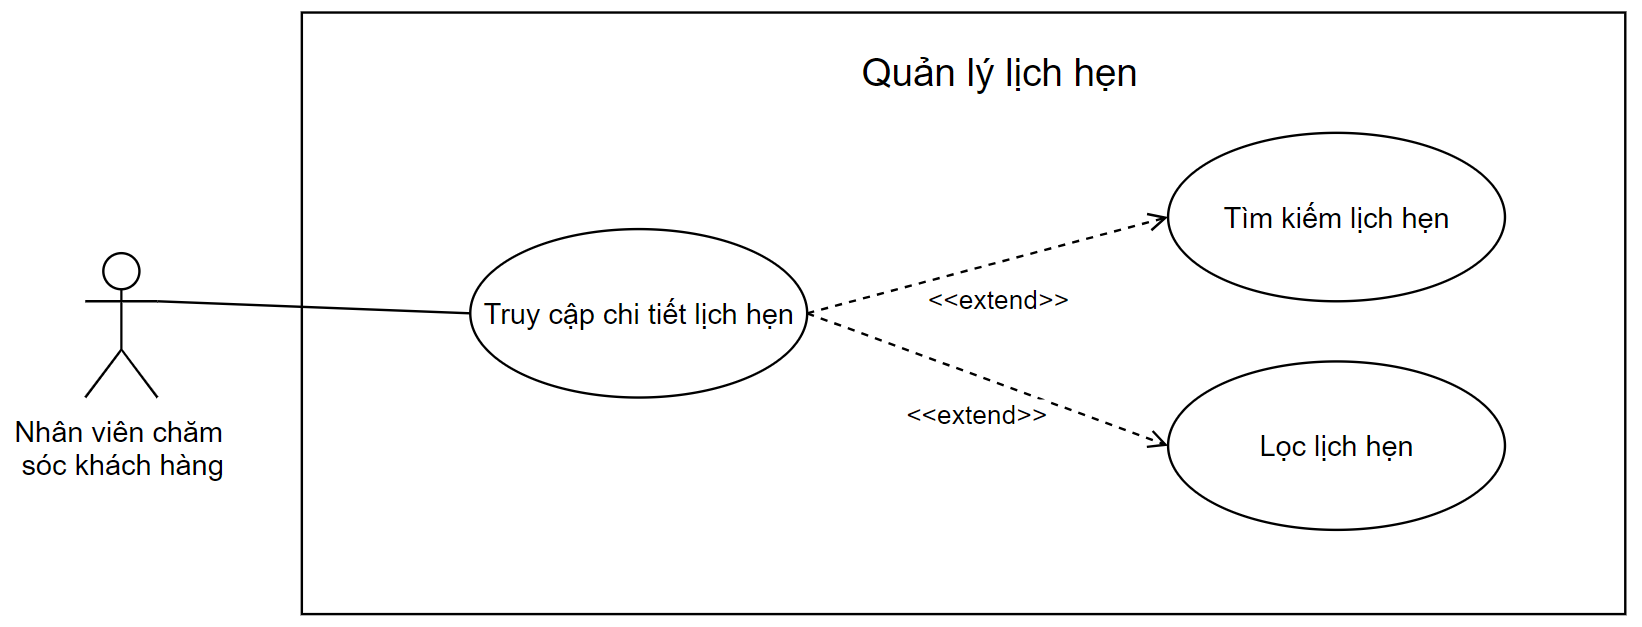
\includegraphics[width=1\linewidth]{Dg_UC/quanlylichhen.png}
    \includesvg[width=1\textwidth]{Dg_UC/Usecase Diagram-AppointmentManagement.drawio.svg}
    \vspace{0.5cm}
    \caption{Biểu đồ use case cho Quản lý lịch hẹn}
    \label{fig:enter-label}
\end{figure}
\subsubsubsection{Use case scenario}
\textbf{Truy cập chi tiết lịch hẹn}
\begin{table}[H]
    \centering
    \begin{tabular}{|l|l|l|l|} 
        \hline
        Use case name: & \multicolumn{3}{|l|}{Truy cập chi tiết lịch hẹn} \\
        \hline
        Created by: & Lê Đình Huy & Last updated by: & Lê Đình Huy \\
        \hline
        Date created: & 19 / 10 / 2024 & Date last updated: & 19 / 10 / 2024 \\
        \hline
        Actors: & \multicolumn{3}{|l|}{Nhân viên chăm sóc khách hàng} \\
        \hline
        Description: & \multicolumn{3}{|p{12cm}|}{Cho phép nhân viên CSKH truy cập và xem chi tiết lịch hẹn.} \\ 
        \hline
        Trigger: & \multicolumn{3}{|p{12cm}|}{Chọn "Lịch hẹn" trên thanh điều hướng.} \\
        \hline
        Preconditions: & \multicolumn{3}{|p{12cm}|}{- Nhân viên có tài khoản trên website. \newline
        - Nhân viên đã đăng nhập thành công vào hệ thống. \newline
        - Thiết bị của nhân viên có kết nối mạng và kết nối với hệ thống. \newline
        - Nhân viên có quyền thực hiện chức năng.} \\
        \hline
        Postconditions: & \multicolumn{3}{|p{12cm}|}{Hệ thống hiển thị chi tiết thông tin lịch hẹn mà khách hàng đã đặt.} \\
        \hline
        Normal Flows: & \multicolumn{3}{|p{12cm}|}{1. Nhân viên CSKH chọn "Lịch hẹn" trên thanh điều hướng.\newline
        2. Hệ thống hiển thị danh sách các lịch hẹn.\newline
        3. Nhân viên CSKH chọn xem một lịch hẹn.\newline
        4. Hệ thống hiển thị chi tiết thông tin lịch hẹn mà khách hàng đã đặt.}\\
        \hline
        Alternative Flows: & \multicolumn{3}{|p{12cm}|}{
        \textbf{A1: Tại bước 3}\newline
        3.1. Nhân viên CSKH chọn vào ô Tìm kiếm và nhập nội dung cần tìm.\newline
        3.2. Nhân viên CSKH chọn "Tìm".\newline
        Tiếp tục bước 2 trong Normal flows.\newline
        \textbf{A2: Tại bước 3}\newline
        3.1. Nhân viên CSKH chọn "Lọc".\newline
        3.2. Hệ thống hiển thị các thông số cho phép của bộ lọc.\newline
        3.3. Nhân viên CSKH chọn một thông số.\newline
        Tiếp tục bước 2 trong Normal flows.} \\
        \hline
        Exceptions: & \multicolumn{3}{|p{12cm}|}{
        \textbf{E1: Tại bước 3 hoặc sau bước 4}\newline
        3.1. Nhân viên CSKH chọn "Hỗ trợ".\newline
        3.2. Hệ thống chuyển đến trang hội thoại với khách hàng.\newline
        Use case dừng lại.
        } \\
        \hline
        Note and issues: & \multicolumn{3}{|p{12cm}|}{Không có} \\
        \hline
    \end{tabular}
    \caption{Use case scenario cho Truy cập chi tiết lịch hẹn}
\end{table}

%-------------------------------------------------------------------

\subsection{Biểu đồ Activity}
\subsubsection{Quản lý tài khoản}
\subsubsubsection{Đăng ký}
\begin{figure}[H]
    \centering
     \includesvg[width=1\textwidth]{Dg_Activity/ManageAccount_Signup.svg}
    \vspace{0.5cm}
    \caption{Biểu đồ activity cho Đăng ký}
    \label{fig:enter-label}
\end{figure}
\subsubsubsection{Đăng nhập}
\begin{figure}[H]
    \centering
     \includesvg[width=1\textwidth]{Dg_Activity/ManageAccount_Login.svg}
    \vspace{0.5cm}
    \caption{Biểu đồ activity cho Đăng nhập}
    \label{fig:enter-label}
\end{figure}
\subsubsubsection{Chỉnh sửa hồ sơ cá nhân}
\begin{figure}[H]
    \centering
     \includesvg[width=1\textwidth]{Dg_Activity/ManageAccount_Profile.svg}
    \vspace{0.5cm}
    \caption{Biểu đồ activity cho Chỉnh sửa hồ sơ cá nhân}
    \label{fig:enter-label}
\end{figure}
\subsubsection{Tích hợp}
\begin{figure}[H]
    \centering
     \includesvg[width=1\textwidth]{Dg_Activity/Activity Diagram-Integration.drawio.svg}
    \vspace{0.5cm}
    \caption{Biểu đồ activity cho Tích hợp}
    \label{fig:enter-label}
\end{figure}
\subsubsection{Quản lý chatbot}
\subsubsubsection{Báo cáo}
\begin{figure}[H]
    \centering
     \includesvg[width=1\textwidth]{Dg_Activity/Report.svg}
    \vspace{0.5cm}
    \caption{Biểu đồ activity cho Báo cáo}
    \label{fig:enter-label}
\end{figure}
\textbf{Mô tả:}
Ban đầu quản trị viên doanh nghiệp chọn vào nút "Báo cáo" trên thanh điều hướng. Khi đó màn hình sẽ chuyển qua trang Báo cáo và hiển thị các thông số và biểu đồ.
\begin{itemize}
    \item Nếu quản trị viên chọn "Lọc", hệ thống sẽ hiển thị các thông số lọc và quản trị viên chọn một thông số. Khi đó, hệ thống sẽ hiển thị lại các thông số và biểu đồ tương ứng với thông số lọc đó. Rồi sau đó quản trị viên có thể chọn "Lọc" tiếp hoặc chọn "Xuất" hoặc dừng lại.
    \item Nếu quản trị viên chọn "Xuất", hệ thống sẽ hiển thị 2 loại tệp. Sau đó người dùng sẽ phải chọn một và chọn "Xem trước". Hệ thống sẽ hiển thị chế độ xem trước file dưới dạng popup. Nếu người dùng chọn "Tải xuống" thì file sẽ được tải về thiết bị. Còn nếu người dùng chọn "Hủy bỏ" thì hệ thống sẽ đóng popup xem trước.
    \item Nếu quản trị viên không chọn gì thì sẽ kết thúc.
\end{itemize}
\subsubsubsection{Lịch sử hội thoại}
\begin{figure}[H]
    \centering
     \includesvg[width=1\textwidth]{Dg_Activity/Chat.svg}
    \vspace{0.5cm}
    \caption{Biểu đồ activity cho Lịch sử hội thoại}
    \label{fig:enter-label}
\end{figure}
\textbf{Mô tả:}
Ban đầu quản trị viên doanh nghiệp chọn vào nút "Chat" trên thanh điều hướng. Khi đó màn hình sẽ chuyển qua trang Chat và hiển thị danh sách các cuộc hội thoại của khách hàng.
\begin{itemize}
    \item Nếu quản trị viên chọn vào ô tìm kiếm, nhập nội dung tìm kiếm và chọn "Tìm" thì khi đó hệ thống sẽ hiển thị các cuộc hội thoại có tên tương ứng với nội dung tìm kiếm.
    \item Nếu quản trị viên chọn "Lọc", hệ thống sẽ hiển thị các thông số lọc và quản trị viên chọn một thông số. Khi đó, hệ thống sẽ hiển thị lại các cuộc hội thoại tương ứng với thông số lọc đó. 
    \item Nếu quản trị viên chọn "Cần hỗ trợ" thì hệ thống sẽ chỉ hiển thị các cuộc hội thoại mà khách hàng đã gửi yêu cầu hỗ trợ.
\end{itemize}

Sau đó quản trị viên có thể lặp lại các bước trên hoặc chọn xem một cuộc hội thoại. Khi quản trị viên chọn xem một cuộc hội thoại thì hệ thống sẽ hiển thị chi tiết cuộc hội thoại đó.
\subsubsection{Thông báo và cảnh báo}
\begin{figure}[H]
    \centering
     \includesvg[width=1\textwidth]{Dg_Activity/Activity Diagram-Notifications and Alerts.drawio.svg}
    \vspace{0.5cm}
    \caption{Biểu đồ activity cho Thông báo và cảnh báo}
    \label{fig:enter-label}
\end{figure}
\subsubsection{Quản lý thanh toán}
\begin{figure}[H]
    \centering
     \includesvg[width=1\textwidth]{Dg_Activity/Activity Diagram-Subscription.drawio.svg}
    \vspace{0.5cm}
    \caption{Biểu đồ activity cho Quản lý thanh toán}
    \label{fig:enter-label}
\end{figure}
\subsubsection{Tương tác với chatbot}
\subsubsubsection{Phản hồi tin nhắn khách hàng}
\begin{figure}[H]
    \centering
     \includesvg[width=1\textwidth]{Dg_Activity/ReplyCustomerMessage.svg}
    \vspace{0.5cm}
    \caption{Biểu đồ activity cho Phản hồi tin nhắn khách hàng}
    \label{fig:enter-label}
\end{figure}
\textbf{Mô tả:}
Ban đầu quản trị viên doanh nghiệp chọn xem đoạn hội thoại của khách hàng tại trang Chat. Hệ thống sẽ hiển thị màn hình chat với khách hàng đó.
\begin{itemize}
    \item Nếu muốn điền hoặc chỉnh sửa tin nhắn, quản trị viên chọn vào khung điền tin nhắn và nhập nội dung tin nhắn. Khi đó hệ thống sẽ hiển thị đoạn tin nhắn mà quản trị viên đã nhập.
    \item Nếu muốn đính kèm tệp, quản trị viên chọn "Đính kèm tệp đa phương tiện". Khi đó, khung chọn tệp từ thiết bị sẽ được hiển thị. Quản trị viên chọn một tệp và chọn "Tải lên". Hệ thống hiển thị tệp được chọn trên màn hình.
    \item Nếu muốn xóa tệp đã tải lên, quản trị viên chọn "Xóa". Khi đó tệp đó sẽ được xóa khỏi màn hình.
\end{itemize}
Sau đó quản trị viên có thể lặp lại các bước trên. Hoặc nếu đã có tin nhắn và quản trị viên chọn gửi thì hệ thống sẽ hiển thị tin nhắn vừa gửi lên màn hình. Hoặc nếu chưa có tin nhắn thì sẽ dừng lại.
\subsubsubsection{Gửi tin nhắn}
\begin{figure}[H]
    \centering
     \includesvg[width=1\textwidth]{Dg_Activity/SendMessage.svg}
    \vspace{0.5cm}
    \caption{Biểu đồ activity cho Gửi tin nhắn}
    \label{fig:enter-label}
\end{figure}
\textbf{Mô tả:}
Ban đầu khách hàng chọn vào chatbot tại màn hình website của doanh nghiệp. Hệ thống sẽ hiển thị màn hình chatbot.
\begin{itemize}
    \item Nếu muốn điền hoặc chỉnh sửa tin nhắn, khách hàng chọn vào khung điền tin nhắn và nhập nội dung tin nhắn. Khi đó hệ thống sẽ hiển thị đoạn tin nhắn mà khách hàng đã nhập.
    \item Nếu muốn đính kèm tệp, khách hàng chọn "Đính kèm tệp đa phương tiện". Khi đó, khung chọn tệp từ thiết bị sẽ được hiển thị. khách hàng chọn một tệp và chọn "Tải lên". Hệ thống hiển thị tệp được chọn trên màn hình.
    \item Nếu muốn xóa tệp đã tải lên, khách hàng chọn "Xóa". Khi đó tệp đó sẽ được xóa khỏi màn hình.
\end{itemize}
Sau đó khách hàng có thể lặp lại các bước trên. Hoặc nếu đã có tin nhắn và khách hàng chọn gửi thì hệ thống sẽ hiển thị tin nhắn vừa gửi lên màn hình. Đồng thời, hệ thống sẽ tạo và gửi lại tin nhắn phản hồi từ AI Chatbot. Hoặc nếu chưa có tin nhắn thì sẽ dừng lại.
\subsubsubsection{Yêu cầu hỗ trợ}
\begin{figure}[H]
    \centering
    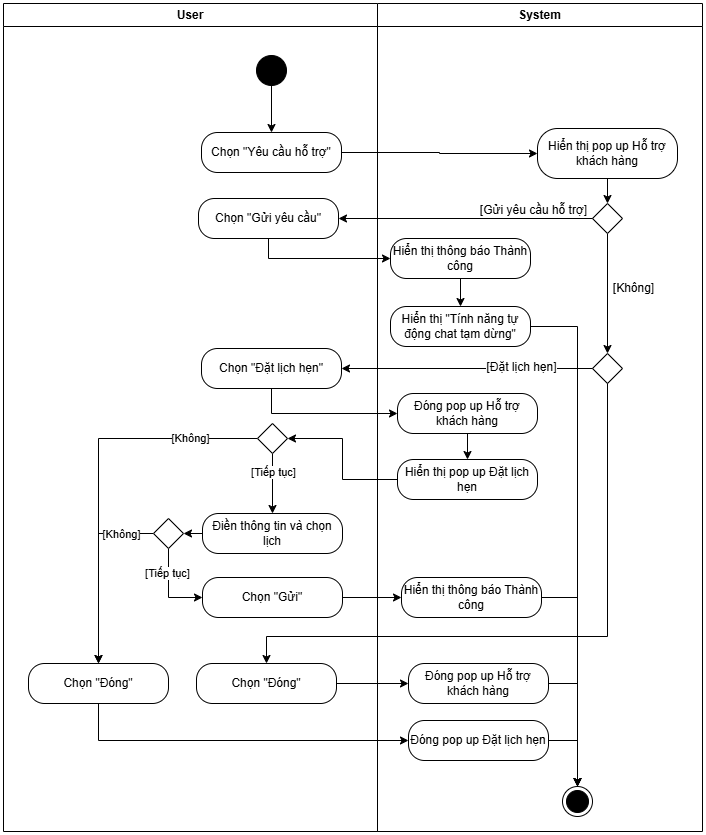
\includegraphics[width=1\textwidth]{Dg_Activity/NeedSupport.png}
    \vspace{0.5cm}
    \caption{Biểu đồ activity cho Yêu cầu hỗ trợ}
    \label{fig:enter-label}
\end{figure}
\textbf{Mô tả:}
Tại màn hình chatbot, khách hàng chọn "Yêu cầu hỗ trợ". Hệ thống sẽ hiển thị popup hỗ trợ khách hàng.
\begin{itemize}
    \item Nếu muốn gửi yêu cầu hỗ trợ, khách hàng chọn "Gửi yêu cầu". Hệ thống sẽ hiển thị thông báo thành công. Khi đó, tính năng tự động chat sẽ tạm dừng.
    \item Nếu muốn đặt lịch hẹn, khách hàng chọn "Đặt lịch hẹn". Hệ thống sẽ đóng popup Hỗ trợ khách hàng và hiển thị popup Đặt lịch hẹn. 
    \begin{itemize}
        \item Nếu muốn tiếp tục, khách hàng điền thông tin và chọn lịch.
        \begin{itemize}
            \item Nếu muốn tiếp tục, khách hàng chọn "Gửi". Hệ thống sẽ hiển thị thông báo thành công.
            \item Nếu không, khách hàng chọn "Đóng".
        \end{itemize}
        \item Nếu không, khách hàng chọn "Đóng".
    \end{itemize}
    Nếu khách hàng chọn "Đóng" thì hệ thống sẽ đóng popup Đặt lịch hẹn.
    \item Nếu khách hàng chọn "Đóng", hệ thống sẽ đóng popup Hỗ trợ khách hàng.
\end{itemize}
\subsubsection{Quản lý lịch hẹn}
\begin{figure}[H]
    \centering
    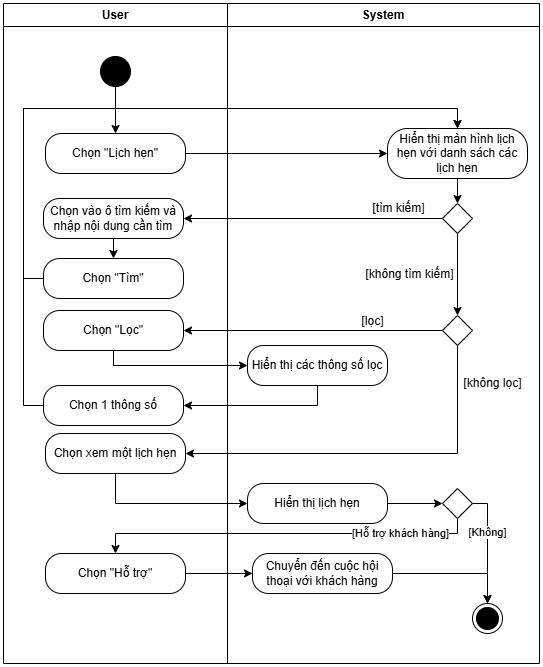
\includegraphics[width=1\textwidth]{Dg_Activity/AppointmentManagement.png}
    \vspace{0.5cm}
    \caption{Biểu đồ activity cho Quản lý lịch hẹn}
    \label{fig:enter-label}
\end{figure}
\textbf{Mô tả:}
Ban đầu quản trị viên doanh nghiệp chọn vào nút "Lịch hẹn" trên thanh điều hướng. Khi đó màn hình sẽ chuyển qua trang Lịch hẹn và hiển thị danh sách các lịch hẹn của khách hàng.
\begin{itemize}
    \item Nếu quản trị viên chọn vào ô tìm kiếm, nhập nội dung tìm kiếm và chọn "Tìm" thì khi đó hệ thống sẽ hiển thị các lịch hẹn có tên tương ứng với nội dung tìm kiếm.
    \item Nếu quản trị viên chọn "Lọc", hệ thống sẽ hiển thị các thông số lọc và quản trị viên chọn một thông số. Khi đó, hệ thống sẽ hiển thị lại các lịch hẹn tương ứng với thông số lọc đó. 
\end{itemize}
Sau đó quản trị viên có thể lặp lại các bước trên hoặc chọn xem một lịch hẹn. Khi quản trị viên chọn xem một lịch hẹn thì hệ thống sẽ hiển thị chi tiết lịch hẹn đó. Ở đó, nếu quản trị viên chọn "Hỗ trợ", hệ thống sẽ chuyển đến cuộc hội thoại với khách hàng. Nếu không thì sẽ dừng lại.




\subsection{Biểu đồ Sequence}
\subsubsection{Quản lý tài khoản}
\subsubsubsection{Đăng ký}
\begin{figure}[H]
	\centering
	\includesvg[width=1\textwidth]{Dg_Sequence/Signupseq.svg}
	\vspace{0.5cm}
	\caption{Biểu đồ sequence cho Đăng ký}
	\label{fig:enter-label}
\end{figure}
\subsubsubsection{Đăng nhập}
\begin{figure}[H]
	\centering
	\includesvg[width=1\textwidth]{Dg_Sequence/Loginseq.svg}
	\vspace{0.5cm}
	\caption{Biểu đồ sequence cho Đăng nhập}
	\label{fig:enter-label}
\end{figure}
\subsubsubsection{Chỉnh sửa hồ sơ cá nhân}
\begin{figure}[H]
	\centering
	\includesvg[width=1\textwidth]{Dg_Sequence/ManageProfileseq.svg}
	\vspace{0.5cm}
	\caption{Biểu đồ sequence cho Chỉnh sửa hồ sơ cá nhân}
	\label{fig:enter-label}
\end{figure}

\subsubsection{Quản lý chatbot}
\subsubsubsection{Báo cáo}
\begin{figure}[H]
    \centering
     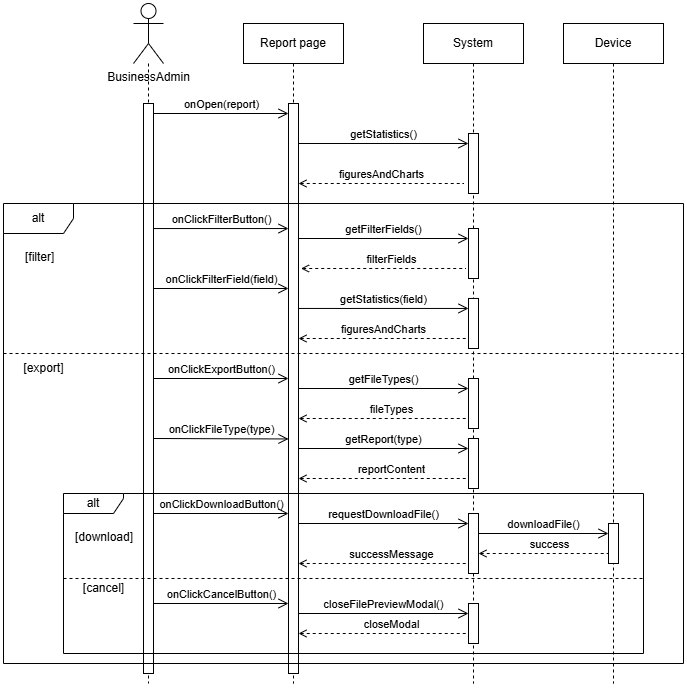
\includegraphics[width=1\textwidth]{Dg_Sequence/Report.png}
    \vspace{0.5cm}
    \caption{Biểu đồ sequence cho Báo cáo}
    \label{fig:enter-label}
\end{figure}
\subsubsubsection{Lịch sử hội thoại}
\begin{figure}[H]
    \centering
     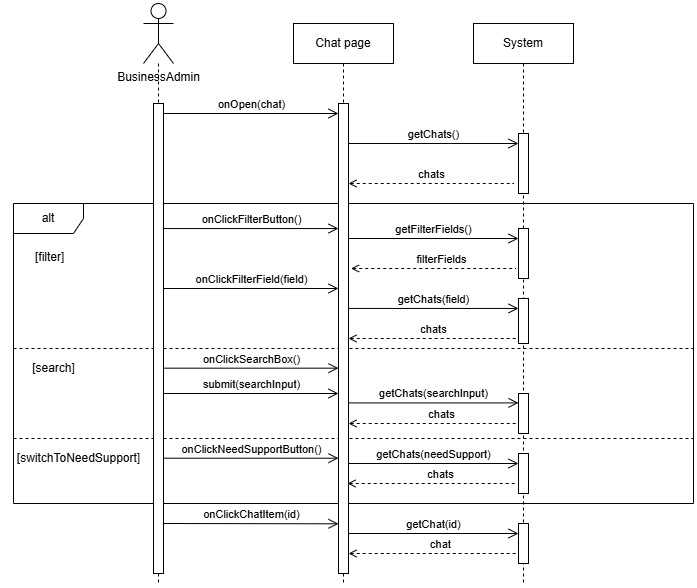
\includegraphics[width=1\textwidth]{Dg_Sequence/Chat.png}
    \vspace{0.5cm}
    \caption{Biểu đồ sequence cho Lịch sử hội thoại}
    \label{fig:enter-label}
\end{figure}

\subsubsection{Quản lý thanh toán}
\begin{figure}[H]
    \centering
     \includesvg[width=1\textwidth]{Dg_Sequence/Payment.svg}
    \vspace{0.5cm}
    \caption{Biểu đồ sequence cho Quản lý thanh toán}
    \label{fig:enter-label}
\end{figure}
\subsubsection{Tương tác với chatbot}
\subsubsubsection{Phản hồi tin nhắn khách hàng}
\begin{figure}[H]
    \centering
     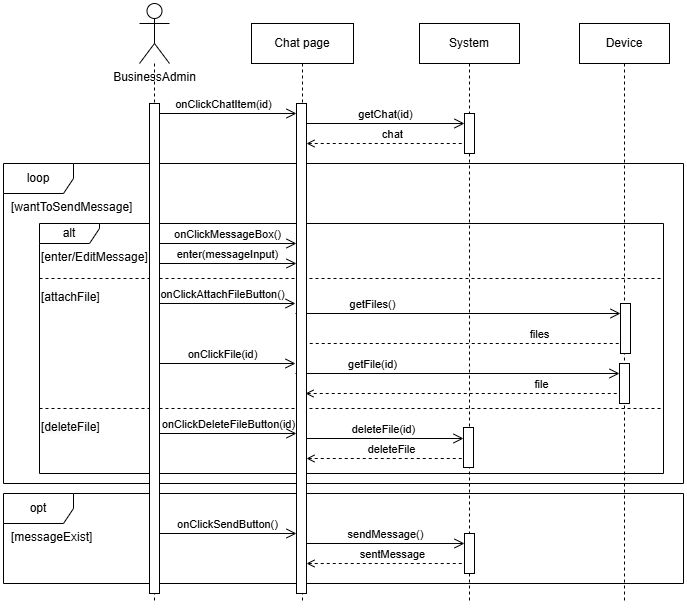
\includegraphics[width=1\textwidth]{Dg_Sequence/ReplyCustomerMessage.png}
    \vspace{0.5cm}
    \caption{Biểu đồ sequence cho Phản hồi tin nhắn khách hàng}
    \label{fig:enter-label}
\end{figure}
\subsubsubsection{Gửi tin nhắn}
\begin{figure}[H]
    \centering
     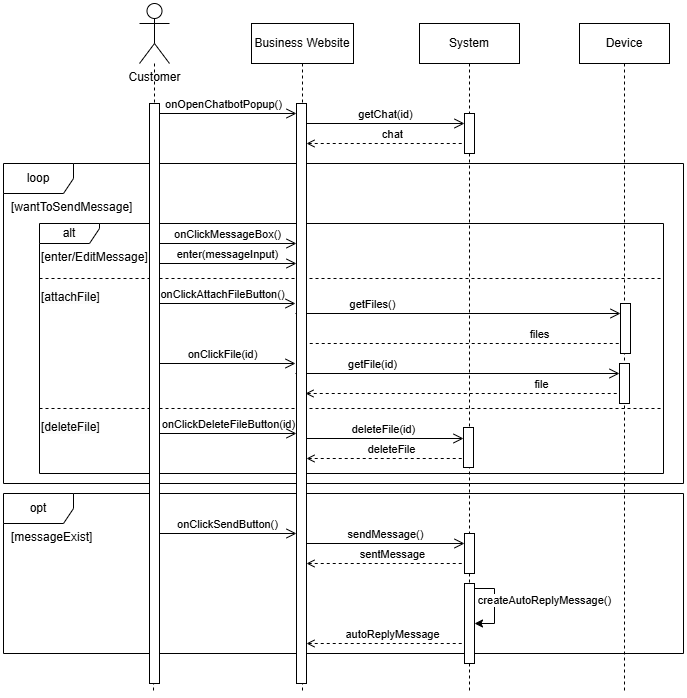
\includegraphics[width=1\textwidth]{Dg_Sequence/SendMessage.png}
    \vspace{0.5cm}
    \caption{Biểu đồ sequence cho Gửi tin nhắn}
    \label{fig:enter-label}
\end{figure}

\subsubsubsection{Yêu cầu hỗ trợ}
\begin{figure}[H]
    \centering
     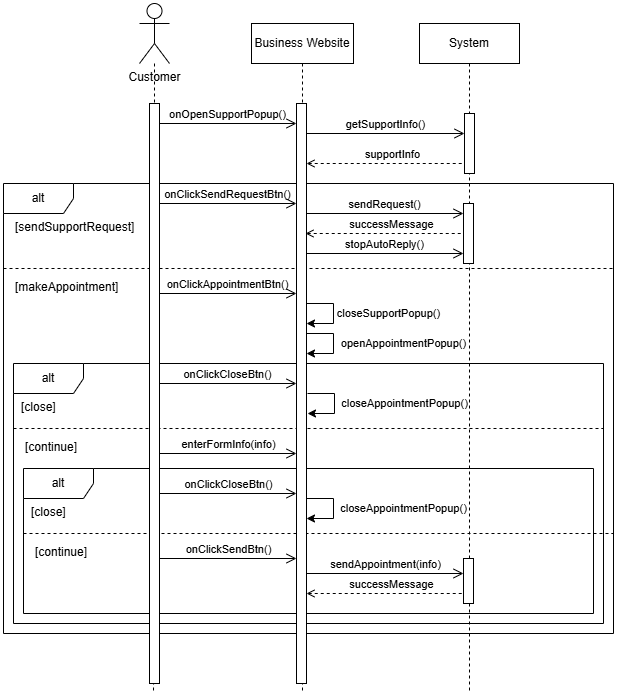
\includegraphics[width=1\textwidth]{Dg_Sequence/NeedSupport.png}
    \vspace{0.5cm}
    \caption{Biểu đồ sequence cho Yêu cầu hỗ trợ}
    \label{fig:enter-label}
\end{figure}
\subsubsection{Quản lý lịch hẹn}
\begin{figure}[H]
    \centering
     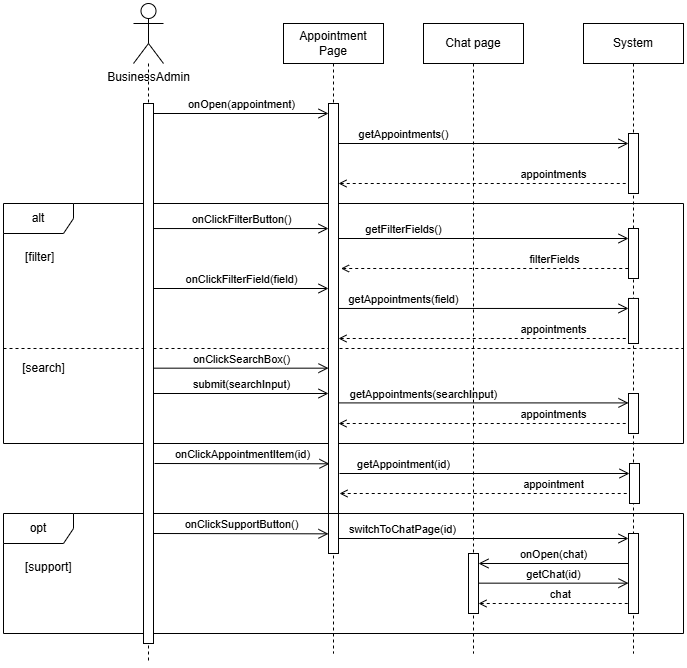
\includegraphics[width=1\textwidth]{Dg_Sequence/AppointmentManagement.png}
    \vspace{0.5cm}
    \caption{Biểu đồ sequence cho Quản lý lịch hẹn}
    \label{fig:enter-label}
\end{figure}

\subsubsection{Đào tạo và tùy chỉnh chatbot}
\subsubsubsection{Tải dữ liệu tri thức}
\begin{figure}[H]
	\centering
	\includesvg[width=1\textwidth]{Dg_Sequence/LoadKnowledgeseq.svg}
	\vspace{0.5cm}
	\caption{Biểu đồ sequence cho Tải dữ liệu tri thức}
	\label{fig:enter-label}
\end{figure}
\subsubsubsection{Cập nhật dữ liệu tri thức}
\begin{figure}[H]
	\centering
	\includesvg[width=1\textwidth]{Dg_Sequence/ModifyKnowledge1.svg}
	\vspace{0.5cm}
	\caption{Biểu đồ sequence cho Cập nhật dữ liệu tri thức}
	\label{fig:enter-label}
\end{figure}
\begin{figure}[H]
	\centering
	\includesvg[width=1\textwidth]{Dg_Sequence/ModifyKnowledge2.svg}
	\vspace{0.5cm}
	\caption{Biểu đồ sequence cho Cập nhật websites}
	\label{fig:enter-label}
\end{figure}
\subsubsubsection{Gán nhãn dữ liệu tri thức}
\begin{figure}[H]
	\centering
	\includesvg[width=1\textwidth]{Dg_Sequence/AssignTopicseq.svg}
	\vspace{0.5cm}
	\caption{Biểu đồ sequence cho Gán nhãn dữ liệu tri thức}
	\label{fig:enter-label}
\end{figure}
\subsubsubsection{Tùy chỉnh chatbot}
\begin{figure}[H]
	\centering
	\includesvg[width=1\textwidth]{Dg_Sequence/AdjustBotseq.svg}
	\vspace{0.5cm}
	\caption{Biểu đồ sequence cho Tùy chỉnh chatbot}
	\label{fig:enter-label}
\end{figure}


\subsection{Biểu đồ Class}
\begin{figure}[H]
    \centering
     \includesvg[width=1\textwidth]{Dg_Activity/ManageAccount_Signup.svg}
    \vspace{0.5cm}
    \caption{Biểu đồ activity cho Đăng ký}
    \label{fig:enter-label}
\end{figure}
